\documentclass[11pt, twoside, fleqn]{report}

\usepackage[backend=biber, style=ieee]{biblatex}
\usepackage[labelfont=bf]{caption}
\usepackage[margin=1in]{geometry}
\usepackage[colorlinks]{hyperref}
\usepackage[version=4]{mhchem}
\usepackage[parfill, skip=1em]{parskip}
\usepackage{amssymb, booktabs, derivative, fancyhdr, float, graphicx, natex, pgfplots, physics2, siunitx, tikz}

% must be loaded after amsmath
\usepackage[capitalize]{cleveref}
% load after xcolor
\usepackage{pagecolor}

% background and foreground colors
\definecolor{bgcolor}{HTML}{1e1e2e}
\definecolor{fgcolor}{HTML}{cdd6f4}

% catppuccin palette
\definecolor{p1}{HTML}{cba6f7}
\definecolor{p2}{HTML}{f38ba8}
\definecolor{p3}{HTML}{fab387}
\definecolor{p4}{HTML}{a6e3a1}
\definecolor{p5}{HTML}{89dceb}
\definecolor{p6}{HTML}{89b4fa}

% siunitx
\DeclareSIUnit{\angstrom}{\text{Å}}

% physics2
\usephysicsmodule{ab}

% pagecolor
\pagecolor{bgcolor}
\color{fgcolor}

% biblatex
\addbibresource{references.bib}

% fancyhdr
\setlength{\headheight}{14pt}
\renewcommand{\chaptermark}[1]{\markboth{\thechapter\ #1}{}}
\renewcommand{\sectionmark}[1]{\markright{\thesection\ #1}}
\renewcommand{\footrulewidth}{0.4pt}

\fancypagestyle{mystyle}{
    \fancyfoot{}
    \fancyfoot[C]{\thepage}
}

% hyperref
\hypersetup{
    linkcolor = p1,
    urlcolor = p2,
    citecolor = p3
}

% pgfplots
\pgfplotsset{compat=newest}

% custom
\newcommand{\dash}{\!-\!}
\newcommand{\state}[2]{\prescript{#1}{}{#2}}

\begin{document}

\pagestyle{empty}

\begin{titlepage}
    \null
    \vspace{\fill}
    \begin{center}
        \let \footnote \thanks
        {\LARGE \textbf{pyGEONOSIS} \par}
        {\large Python GEnerated Oxygen and Nitric Oxide SImulated Spectra}
        \vskip 1.5em
            {\large
                \lineskip .5em
                \begin{tabular}[t]{c}
                    Nathan Phillips
                \end{tabular}\par}
        \vskip 1em
            {\large \today}
        \vskip 2em
    \end{center}
    \vspace{\fill}

    \begin{center}
        {\large{\textbf{Texas A\&M University}} \par}
        {\large{Department of Aerospace Engineering}}
    \end{center}
\end{titlepage}

\tableofcontents
\newpage
\listoffigures
\newpage
\listoftables
\newpage

\pagestyle{mystyle}

\chapter{Molecular Approximations}
\label{c:molecular_approximations}

\section{The Rigid Rotator}
\label{s:the_rigid_rotator}

\subsection{Theory}

The rigid rotator model assumes that the molecule is shaped like a dumbbell. Each of the two atoms of masses $m_1$ and $m_2$ is point-like and are affixed to one another via a massless rigid rod of radius $r$.

\begin{figure}[H]
    \centering
    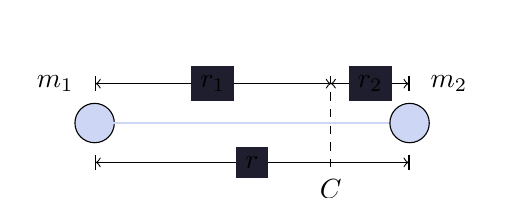
\begin{tikzpicture}
        \draw[fill=fgcolor](-2,0) circle(0.25);
        \node at (-2.5,0.5){$m_1$};
        \draw[color=fgcolor] (-2,0)rectangle(2,0);
        \draw[fill=fgcolor] (2,0)circle(0.25);
        \node at (2.5,0.5){$m_2$};

        \draw[|<->|](-2,-0.5)--(2,-0.5) node[midway, fill=bgcolor]{$r$};
        \draw[dashed](1,0.6)--(1,-0.6) node[below]{$C$};
        \draw[|<->](-2,0.5)--(1,0.5) node[midway, fill=bgcolor]{$r_1$};
        \draw[<->|](1,0.5)--(2,0.5) node[midway, fill=bgcolor]{$r_2$};
    \end{tikzpicture}
    \caption{Dumbbell model of a diatomic molecule.}
    \label{f:dumbbell_model}
\end{figure}

The classical expression for the rotational energy of a rigid body is
\begin{equation*}
    E = \frac{1}{2}I\omega^2,
\end{equation*}
where $\omega$ is the angular velocity and $I$ is the moment of inertia of the body about the axis of rotation $C$. For a point mass, the moment of inertia about an axis of a body is
\begin{equation*}
    I = \sum_i m_i r_i^2.
\end{equation*}
Using this definition, the magnitude of the angular momentum of the system can be found as
\begin{equation*}
    L = I\omega.
\end{equation*}
Using the angular momentum, the rotational energy of the system can now be expressed as
\begin{equation*}
    E = \frac{L^2}{2I}.
\end{equation*}

For the dumbbell model, the moment of inertia is
\begin{equation*}
    I = m_1r_1^2 + m_2r_2^2,
\end{equation*}
where
\begin{equation*}
    r_1 = \frac{m_2}{m_1 + m_2}r \quad\text{and}\quad r_2 = \frac{m_1}{m_1 + m_2}r
\end{equation*}
are the distances of the two masses $m_1$ and $m_2$ from the center of gravity $C$. Substituting these two expressions into the moment of inertia gives
\begin{equation*}
    I = \mu r^2,
\end{equation*}
where
\begin{equation*}
    \mu = \frac{m_1m_2}{m_1 + m_2}
\end{equation*}
is the reduced mass of the molecule.

\subsection{Energy Levels}

The appropriate Schr\"odinger Equation for the rigid rotator has $m = \mu$ and $V = 0$ since the model is regarded as perfectly rigid. Solving
\begin{equation*}
    \odv[2]{\psi}{x} + \pdv[2]{\psi}{y} + \pdv[2]{\psi}{z} + \frac{8\pi^2\mu}{h^2}E\psi = 0
\end{equation*}
leads to the energy eigenvalues given by
\begin{equation*}
    E = \frac{h^2J(J + 1)}{8\pi^2\mu r^2} = \frac{h^2J(J + 1)}{8\pi^2I},
\end{equation*}
where $J$ is the rotational quantum number. The quantized angular momentum can be found using the classical formula shown earlier, which leads to
\begin{equation*}
    L = \sqrt{2EI} = \frac{h}{2\pi}\sqrt{J(J + 1)}.
\end{equation*}
The angular velocity $\omega$ and rotational frequency $\nu\_{rot}$ can also be found as
\begin{equation*}
    \omega = \frac{h}{2\pi I}\sqrt{J(J + 1)} \quad\text{and}\quad \nu\_{rot} = \frac{\omega}{2\pi} = \frac{h}{4\pi^2I}\sqrt{J(J + 1)}.
\end{equation*}

\subsection{Spectrum}

The emission of a light quantum results from the transition of the rotator from a higher to a lower energy level. Conversely, the absorption of a light quantum produces a transition from a lower to a higher level. The wave number $\nu$ of the emitted or absorbed quantum is
\begin{equation*}
    \nu = \frac{E'}{hc} - \frac{E''}{hc}.
\end{equation*}
The single prime $'$ refers to the upper state, while the double prime $''$ refers to the lower state.

The quantity $E/hc$ is called the rotational term value and is denoted $F(J)$. The value of $F(J)$ is given as
\begin{equation*}
    F(J) = \frac{E}{hc} = \frac{h}{8\pi^2cI}J(J + 1) = BJ(J + 1).
\end{equation*}
The constant
\begin{equation*}
    B = \frac{h}{8\pi^2cI}
\end{equation*}
is called the rotational constant and is essentially the reciprocal moment of inertia. These two definitions allow for the rewriting of the wavenumber as
\begin{equation*}
    \nu = F(J')- F(J'') = BJ'(J' + 1) - BJ''(J'' + 1).
\end{equation*}

To find which frequencies are actually emitted or absorbed, selection rules for the rotational quantum number $J$ must be established. The selection rule for $J$ is
\begin{equation*}
    J' = J'' \pm 1; \quad\text{that is,}\quad \Delta{}J = J' - J'' = \pm 1.
\end{equation*}

Because $J' > J''$ always (due to $J'$ being the upper state), only $\Delta{}J = +1$ needs to be considered. Therefore, the absorbed or emitted lines of the rigid rotator are given by
\begin{equation*}
    \nu = F(J'' + 1) - F(J'') = B(J'' + 1)(J'' + 2) - BJ''(J'' + 1) = 2B(J'' + 1).
\end{equation*}
Writing $J$ instead of $J''$ when only the $J$ value of the lower state occurs, we get
\begin{equation*}
    \nu = 2B(J + 1) \quad\text{for}\quad J = 0, 1, 2, \dotsb.
\end{equation*}
The rotational frequency of the rigid rotator is
\begin{equation*}
    \nu\_{rot} = 2cB\sqrt{J(J + 1)}.
\end{equation*}

\section{The Harmonic Oscillator}
\label{s:the_harmonic_oscillator}

\subsection{Theory}

In classical mechanics, the equation of motion for a simple harmonic oscillator is
\begin{equation*}
    F = -kx = m\odv[2]{x}{t},
\end{equation*}
where $F$ is the force experienced by the particle toward the equilibrium position which is proportional to the distance $x$ away from the equilibrium position. Solving the differential equation for $x$ yields
\begin{equation*}
    x = x_0\sin(2\pi t\nu\_{vib} + \varphi),
\end{equation*}
where the vibrational frequency $\nu\_{vib}$ is given by
\begin{equation*}
    \nu\_{vib} = \frac{1}{2\pi}\sqrt{\frac{k}{m}}.
\end{equation*}

The potential energy for a linear spring is
\begin{equation*}
    V = \frac{1}{2}kx^2 = 2\pi^2mx^2\nu\_{vib}^2
\end{equation*}

The restoring force exerted by the two atoms in a molecule after being displaced from their equilibrium position $r_e$ can be modeled by the equation of motion for a spring as
\begin{equation*}
    m_1\odv[2]{r_1}{t} = -k(r - r_e)
\end{equation*}
and
\begin{equation*}
    m_2\odv[2]{r_2}{t} = -k(r - r_e).
\end{equation*}
Substituting $r$ in place of both $r_1$ and $r_2$ gives the single equation
\begin{equation*}
    \frac{m_1m_2}{m_1 + m_2}\odv[2]{r}{t} = -k(r - r_e),
\end{equation*}
which is equivalent to
\begin{equation*}
    \mu\odv[2]{(r - r_e)}{t} = -k(r - r_e)
\end{equation*}
since $r_e$ is constant. From direct comparison with the classical equation of motion for a harmonic oscillator, it follows that the vibrational frequency of the molecule is
\begin{equation*}
    \nu\_{vib} = \frac{1}{2\pi}\sqrt{\frac{k}{\mu}}.
\end{equation*}

\subsection{Energy Levels}

The Schr\"odinger equation for the harmonic oscillator is
\begin{equation*}
    \odv[2]{\psi}{x} + \frac{8\pi^2\mu}{h^2}\ab(E - \tfrac{1}{2}kx^2)\psi = 0.
\end{equation*}
Solving this equation leads to the energy eigenvalues given by
\begin{equation*}
    E(v) = \frac{h}{2\pi}\sqrt{\frac{k}{\mu}}\ab(v + \tfrac{1}{2}) = h\nu\_{vib}\ab(v + \tfrac{1}{2}) \quad\text{for}\quad v = 0, 1, 2, \dotsb.
\end{equation*}
Rewriting the energy as the vibrational term value $G(v)$ gives
\begin{equation*}
    G(v) = \frac{E(v)}{hc} = \frac{\nu\_{vib}}{c}\ab(v + \tfrac{1}{2}) = \omega\ab(v + \tfrac{1}{2}),
\end{equation*}
where the quantity $\nu\_{vib}/c$ is designated $\omega$ and measured in \unit{cm^{-1}}.

\subsection{Spectrum}

Similarly to the rigid rotor, the wavenumber of the emitted or absorbed light is given by
\begin{equation*}
    \nu = \frac{E(v')}{hc} - \frac{E(v'')}{hc} = G(v') - G(v''),
\end{equation*}
where $v'$ and $v''$ are the quantum numbers of the upper and lower state, respectively.

The selection rule for the vibrational quantum number of the harmonic oscillator is
\begin{equation*}
    \Delta{}v = v' - v'' = \pm 1.
\end{equation*}
Again denoting $J''$ as $J$, the wavenumber of the emitted or absorbed light is
\begin{equation*}
    \nu = G(v + 1) - G(v) = \omega.
\end{equation*}

\section{The Anharmonic Oscillator}
\label{s:the_anharmonic_oscillator}

\subsection{Theory}

A first approximation to the actual potential energy function of the molecule can be written as
\begin{equation*}
    U = f(r - r_e)^2 - g(r - r_e)^3,
\end{equation*}
where $f$ and $g$ are coefficients, with $g$ being much smaller than $f$. Better approximations can be made by adding higher order terms to this expression.

The motion of the anharmonic oscillator can be represented as a superposition of fundamental and overtone vibrations as the following Fourier series:
\begin{equation*}
    x = x_{01}\sin{2\pi\nu\_{vib}t} + x_{02}(3 + \cos{2\pi2\nu\_{vib}t}) + x_{03}\sin{2\pi3\nu\_{vib}t} + \dotsb.
\end{equation*}
In this expression, $x_{01}$, $x_{02}$, and $x_{03}$ are the amplitudes of the fundamental, the first, and the second overtone, respectively. If the anharmonicity is small $(g \ll f)$, then $x_{02} \ll x_{01}$ and $x_{03} \ll x_{02}$. However, $x_{02}$ and $x_{03}$ are proportional to the square and cube of $x_{01}$, respectively and rapidly become more important as $x_{01}$ increases. Because of the asymmetric potential curve, the time average of the position is not at $x = 0$, but instead at $x = 3x_{02}$.

The frequency of the vibrations is given as
\begin{equation*}
    \nu\_{vib} = \frac{1}{2\pi}\sqrt{\frac{k}{\mu}}
\end{equation*}
for very small amplitudes only. This factor decreases slowly as the amplitude $x_{01}$ increases.

\subsection{Energy Levels}

Substituting the anharmonic potential energy function into the Schr\"odinger equation and solving for the energy eigenvalues gives
\begin{equation*}
    E_v = hc\omega_e\ab(v + \tfrac{1}{2}) - hc\omega_ex_e\ab(v + \tfrac{1}{2})^2 + hc\omega_ey_e\ab(v + \tfrac{1}{2})^3 + \dotsb.
\end{equation*}
Written as the vibrational term $G(v)$, this becomes
\begin{equation*}
    G(v) = \omega_e\ab(v + \tfrac{1}{2}) - \omega_ex_e\ab(v + \tfrac{1}{2})^2 + \omega_ey_e\ab(v + \tfrac{1}{2})^3 + \dotsb,
\end{equation*}
where $v$ is the vibrational quantum number, $\omega_ex_e \ll \omega_e$, and $\omega_ey_e \ll \omega_ex_e$. This equation directly shows that the energy levels of the anharmonic oscillator are not equidistant like those of the harmonic oscillator.

The zero-point energy of the anharmonic oscillator is given by setting $v = 0$ in the vibrational term above:
\begin{equation*}
    G(0) = \tfrac{1}{2}\omega_e - \tfrac{1}{2}\omega_ex_e + \tfrac{1}{8}\omega_ey_e + \dotsb.
\end{equation*}

\subsection{Spectrum}

The selection rule for the anharmonic oscillator is given by
\begin{equation*}
    \Delta{}v = \pm 1
\end{equation*}
for the most intense transitions, but the two selection rules of
\begin{equation*}
    \Delta{}v = \pm 2 \quad\text{and}\quad \Delta{}v = \pm 3
\end{equation*}
can also appear with decreasing intensity.

The formula for the series of absorption bands $1\dash0$, $2\dash0$, $3\dash0$, $\dotsb$ is given as
\begin{equation*}
    \nu\_{abs} = G(v') - G(0) = G_0(v') = \omega_0v' - \omega_0x_0v'^2 + \omega_0y_0v'^3 + \dotsb.
\end{equation*}

\section{The Nonrigid Rotator}
\label{s:the_nonrigid_rotator}

\subsection{Energy Levels}

A good approximation shows that the rotational terms of the nonrigid rotator are given by
\begin{equation*}
    F(J) = \frac{E_r}{hc} = B[1 - uJ(J + 1)]J(J + 1),
\end{equation*}
where the value $B[1 - uJ(J + 1)]$ now appears in the place of $B$ in the equation for the rigid rotator. This equation can also be written as
\begin{equation*}
    F(J) = BJ(J + 1) - DJ^2(J + 1)^2,
\end{equation*}
where $D$ always has a positive value with this choice of sign. If cubic and higher powers in the potential energy are included, the rotational terms values are
\begin{equation*}
    F(J) = BJ(J + 1) - DJ^2(J + 1)^2 + HJ^3(J + 1)^3 + \dotsb.
\end{equation*}

\subsection{Spectrum}

The selection rule for the infrared spectrum of the rigid rotator $\Delta{}J = \pm 1$ is also valid for the nonrigid rotator. Therefore, the wavenumbers of the lines of the infrared rotation spectrum are
\begin{equation*}
    \nu = F(J + 1) - F(J) = 2B(J + 1) - 4D(J + 1)^3.
\end{equation*}

\section{The Vibrating Rotator}
\label{s:the_vibrating_rotator}

\subsection{Energy Levels}

Since the molecule is vibrating, the internuclear distance and therefore the moment of inertia and the rotational constant $B$ are changing rapidly. Since the period of vibration is small compared to the period of rotation, the mean value of $B$ is
\begin{equation*}
    B_v = \frac{h}{8\pi^2c\mu}\ab[\bar{\frac{1}{r^2}}],
\end{equation*}
where $\overline{1/r^2}$ is the mean value of $1/r^2$ during the vibration. The value of $B_v$ will be expected to be smaller than the equilibrium constant $B_e$ since the mean nuclear separation will be greater. The value of $B_e$ is given by
\begin{equation*}
    B_e = \frac{h}{8\pi^2c\mu{}r_e^2} = \frac{h}{8\pi^2cI_e}.
\end{equation*}
To a first approximation, the rotational constant $B_v$ in the vibrational state $v$ is given as
\begin{equation*}
    B_v = B_e - \alpha_e\ab(v + \tfrac{1}{2}) + \dotsb,
\end{equation*}
where $\alpha_e$ is a constant which is small compared to $B_e$. The ratio $\alpha_e/B_e$ is only slightly larger than $\omega_ex_e/\omega_e$.

A mean rotational constant $D_v$ representing the contribution of centrifugal force can be found as
\begin{equation*}
    D_v = D_e + \beta_e\ab(v + \tfrac{1}{2}) + \dotsb.
\end{equation*}
In this equation, $\beta_e$ is small compared to
\begin{equation*}
    D_e = \frac{4B_e^3}{\omega_e^2}.
\end{equation*}

The rotational terms in a given vibrational level are therefore given by
\begin{equation*}
    F_v(J) = B_vJ(J + 1) - D_vJ^2(J + 1)^2 + \dotsb.
\end{equation*}
Taking into account the interaction between vibration and rotation, the term values for the vibrating rotator are
\begin{equation*}
    T = G(v) + F_v(J) = \omega_e\ab(v + \tfrac{1}{2}) - \omega_ex_e\ab(v + \tfrac{1}{2})^2 + \dotsb + B_vJ(J + 1) - D_vJ^2(J + 1)^2 + \dotsb.
\end{equation*}
For the lowest vibrational state $v = 0$, the rotational constant $B_0$ must be used in this equation.

If very precise measurements are available, higher powers of $\ab(v + \tfrac{1}{2})$ can be taken into account using
\begin{equation*}
    B_v = B_e - \alpha_e\ab(v + \tfrac{1}{2}) + \gamma_e\ab(v + \tfrac{1}{2})^2 + \dotsb.
\end{equation*}
In higher powers of $J(J + 1)$, the rotational term can be expressed as
\begin{equation*}
    F_v(J) = B_vJ(J + 1) - D_vJ^2(J + 1)^2 + H_vJ^3(J + 1)^3 + \dotsb,
\end{equation*}
where the rotational constant $H_v$ is given as
\begin{equation*}
    H_v \approx H_e = \frac{2D_e}{3\omega_e^2}(12B_e^2 - \alpha_e\omega_e)
\end{equation*}
to a first approximation.

\section{The Symmetric Top}
\label{s:the_symmetric_top}

\subsection{Theory}

\subsection{Energy Levels}

\subsection{Spectra}


\chapter{Structure of Electronic Transitions}
\label{c:structure_of_electronic_transitions}

\section{Total Energy}
\label{s:total_energy}

The total energy $E$ of a molecule is approximated by
\begin{equation*}
    E = E_e + E_v + E_r,
\end{equation*}
that is, the sum of the electronic, vibrational, and rotational energy terms. The same equation written in wavenumber units is
\begin{equation}
    T = T_e + G + F.
\end{equation}

\section{Vibrational Term}
\label{s:vibrational_term}

For the vibrational and rotational states of the molecule in different electronic states, the vibrating rotator model is used \cite{herzbergMolecularSpectraMolecular1950}. The fourth-order approximation for the vibrational term $G(v)$ is
\begin{equation}
    G(v) = \omega_e\ab(v + \tfrac{1}{2}) - \omega_ex_e\ab(v + \tfrac{1}{2})^2 + \omega_ey_e\ab(v + \tfrac{1}{2})^3 + \omega_ez_e\ab(v + \tfrac{1}{2})^4 + \dotsb.
\end{equation}

\section{Rotational Term}
\label{s:rotational_term}

The rotational term $F_v(J)$ approximated to the third order is given as
\begin{equation}
    F_v(J) = B_vJ(J + 1) - D_vJ^2(J + 1)^2 + H_vJ^3(J + 1)^3 + \dotsb.
\end{equation}
The rotational constant $B_v$ can be approximated to the third order as (Herz. pp. 108)
\begin{equation*}
    B_v = B_e - \alpha_e\ab(v + \tfrac{1}{2}) + \gamma_e\ab(v + \tfrac{1}{2})^2 + \delta_e\ab(v + \tfrac{1}{2})^3 + \dotsb.
\end{equation*}
The centrifugal distortion constant $D_v$ can be approximated to the first order as (Herz. pp. 107)
\begin{equation}
    D_v = D_e + \beta_e\ab(v + \tfrac{1}{2}) + \dotsb.
\end{equation}
Finally, the third-order constant $H_v$ can be found as the first approximation (Herz. pp. 109)
\begin{equation}
    H_v \approx H_e.
\end{equation}

\section{Transition Wavenumbers}
\label{s:transition_wavenumbers}

The wavenumbers of the spectral lines corresponding to the transitions between two electronic states (in emission or absorption) are given by
\begin{equation}
    \nu = T' - T'' = (T_e' - T_e'') + (G' - G'') + (F' - F'').
\end{equation}
That is, the emitted or absorbed frequencies can be expressed as sums of their constituent parts:
\begin{equation*}
    \nu = \nu_e + \nu_v + \nu_r.
\end{equation*}


\chapter{Intensities in Rotation-Vibration Spectra}
\label{c:intensities_in_rotation-vibration_spectra}

\section{Vibration}
\label{s:vibration}

\subsection{Partition Function}

The quantities given by
\begin{equation*}
    \eul^{-G_0(v)hc/kT}
\end{equation*}
give the relative numbers of molecules in the different vibrational levels relative to the number of molecules in the lowest vibrational level. A more useful equation gives the ratio between the number of molecules in a certain vibrational level relative to the total number of molecules as
\begin{equation*}
    \frac{N_v}{N} = \frac{\eul^{-G_0(v)hc/kT}}{Q_v}.
\end{equation*}
Here, $Q_v$ is the vibrational partition function and is given by
\begin{equation*}
    Q_v = \sum_{v=0}^{\infty}\eul^{-G_0(v)hc/kT} = 1 + \eul^{-G_0(1)hc/kT} + \eul^{-G_0(2)hc/kT} + \dotsb.
\end{equation*}

\subsection{Intensities}

\subsection{Franck-Condon Factors}

\section{Rotation}
\label{s:rotation}

\subsection{Partition Function}

The number of molecules $N_J$ in the rotational level $J$ of the lowest vibrational state at the temperature $T$ is proportional to
\begin{equation*}
    (2J + 1)\eul^{-F(J)hc/kT}.
\end{equation*}
For most practical cases like a rigid rotator with $\Lambda = 0$,
\begin{equation*}
    N_J \propto (2J + 1)\eul^{-BJ(J + 1)hc/kT}.
\end{equation*}
The number of molecules in the different rotational states does not increase linearly and goes through a maximum with the rotational quantum number
\begin{equation*}
    J\_{max} = \sqrt{\frac{kT}{2Bhc}} - \frac{1}{2}.
\end{equation*}

The ratio of the actual number of molecules in a given rotational state is given by
\begin{equation*}
    \frac{N_J}{N} = (2J + 1)\frac{\eul^{-F(J)hc/kT}}{Q_r},
\end{equation*}
where the rotational partition function $Q_r$ is given as
\begin{equation}
    Q_r = \sum_{J=0}^{\infty}(2J + 1)\eul^{-F(J)hc/kT} = 1 + 3\eul^{-F(1)hc/kT} + 5\eul^{-F(2)hc/kT} + \dotsb.
\end{equation}

For higher vibrational levels,
\begin{equation}
    N_J \propto (2J + 1)\eul^{-(G + F)hc/kT}.
\end{equation}
However, the factor $\eul^{-Ghc/kT}$ can be separated off since the distribution over the rotational levels is the same but the absolute population of all the levels is considerably smaller than for the lowest vibrational level.

\subsection{Intensities}

\subsection{H\"onl-London Factors}

\begin{table}[H]
    \centering
    \caption{H\"onl-London factors \cite{herzberg:diatomic}.}
    \label{t:honl-london_factors}
    \begin{tabular}{ccc}
        \toprule
        Branch  & Absorption                                                                & Emission                                                           \\
        \midrule
        \multicolumn{3}{c}{$\adif{\Lambda} = 0$ \textit{Transitions}}                                                                                            \\
        \cmidrule(lr){1-3}
        $S_J^R$ & $\dfrac{(J'' + 1 + \Lambda'')(J'' + 1 - \Lambda'')}{J'' + 1}$             & $\dfrac{(J' + \Lambda')(J' - \Lambda')}{J'}$                       \\
        \addlinespace[0.5em]
        $S_J^Q$ & $\dfrac{(2J'' + 1)\Lambda''^2}{J''(J'' + 1)}$                             & $\dfrac{(2J' + 1)\Lambda'^2}{J'(J' + 1)}$                          \\
        \addlinespace[0.5em]
        $S_J^P$ & $\dfrac{(J'' + \Lambda'')(J'' - \Lambda'')}{J''}$                         & $\dfrac{(J' + 1 + \Lambda')(J' + 1 - \Lambda')}{J' + 1}$           \\
        \addlinespace[0.5em]
        \multicolumn{3}{c}{$\adif{\Lambda} = +1$ \textit{Transitions}}                                                                                           \\
        \cmidrule(lr){1-3}
        $S_J^R$ & $\dfrac{(J'' + 2 + \Lambda'')(J'' + 1 + \Lambda'')}{4(J'' + 1)}$          & $\dfrac{(J' + \Lambda')(J' - 1 + \Lambda')}{4J'}$                  \\
        \addlinespace[0.5em]
        $S_J^Q$ & $\dfrac{(J'' + 1 + \Lambda'')(J'' - \Lambda'')(2J'' + 1)}{4J''(J'' + 1)}$ & $\dfrac{(J' + \Lambda')(J' + 1 - \Lambda')(2J' + 1)}{4J'(J' + 1)}$ \\
        \addlinespace[0.5em]
        $S_J^P$ & $\dfrac{(J'' - 1 - \Lambda'')(J'' - \Lambda'')}{4J''}$                    & $\dfrac{(J' + 1 - \Lambda')(J' + 2 - \Lambda')}{4(J' + 1)}$        \\
        \addlinespace[0.5em]
        \multicolumn{3}{c}{$\adif{\Lambda} = -1$ \textit{Transitions}}                                                                                           \\
        \cmidrule(lr){1-3}
        $S_J^R$ & $\dfrac{(J'' + 2 - \Lambda'')(J'' + 1 - \Lambda'')}{4(J'' + 1)}$          & $\dfrac{(J' - \Lambda')(J' - 1 - \Lambda')}{4J'}$                  \\
        \addlinespace[0.5em]
        $S_J^Q$ & $\dfrac{(J'' + 1 - \Lambda'')(J'' + \Lambda'')(2J'' + 1)}{4J''(J'' + 1)}$ & $\dfrac{(J' - \Lambda')(J' + 1 + \Lambda')(2J' + 1)}{4J'(J' + 1)}$ \\
        \addlinespace[0.5em]
        $S_J^P$ & $\dfrac{(J'' - 1 + \Lambda'')(J'' + \Lambda'')}{4J''}$                    & $\dfrac{(J' + 1 + \Lambda')(J' + 2 + \Lambda')}{4(J' + 1)}$        \\
        \bottomrule
    \end{tabular}
\end{table}

\section{Band Intensity}
\label{s:band_intensity}

The variation of the intensity of the lines in a rotation-vibration band as a function of $J$ is essentially given by the thermal distribution of the rotational levels. In this approximation, it is assumed that the transition probability is the same for all lines of a band. In reality, there is a slight dependence on $J$ and $\Delta{}J$. For the case of $\Lambda = 0$ when only the $P$ and $R$ branches appear, $J' + J'' + 1$ can be used in place of $2J + 1$; that is, the intensity depends on the mean value of $2J + 1$ for the upper and lower states. The $J$ value of the initial state should be used in the exponential term. For absorption, that is $J''$; for emission, $J'$.

The intensities of the lines of rotation or rotation-vibration bands in absorption are
\begin{equation}
    I\_{abs} = \frac{C\_{abs}\nu}{Q_r}(J' + J'' + 1)\eul^{-F(J'')hc/kT}.
\end{equation}
In emission, they are
\begin{equation}
    I\_{em} = \frac{C\_{em}\nu^4}{Q_r}(J' + J'' + 1)\eul^{-F(J')hc/kT}.
\end{equation}


\chapter{Quantum Numbers}
\label{c:quantum_numbers}

\section{Atoms}
\label{s:atoms}

\subsection{Atomic Term Symbol}

\begin{equation*}
    \state{2S + 1}{L_J}
\end{equation*}

\section{Molecules}
\label{s:molecules}

\subsection{Molecular Term Symbol}

\begin{equation*}
    \state{2S + 1}{\Lambda_{\Omega, (g/u)}^{(+/-)}}
\end{equation*}


\chapter{Hund's Coupling Cases}
\label{c:hunds_coupling_cases}

\section{Hund's Case (a)}
\label{s:hunds_case_a}

\subsection{Good Quantum Numbers}

\begin{equation*}
    \Lambda, S, \Sigma, J, \Omega
\end{equation*}

\subsection{Selection Rules}

General rules
\begin{align*}
    g &\nleftrightarrow g, \quad g \leftrightarrow u, \quad u \nleftrightarrow u \\
    \adif{J} &= 0, \pm 1 \text{ with the restriction } J = 0 \nrightarrow J = 0
\end{align*}

Rules common to both (a) and (b)
\begin{align*}
    \adif{\Lambda} &= 0, \pm 1 \\
    \adif{S} &= 0
\end{align*}

Rules for case (a) only
\begin{align*}
    \adif{\Sigma} &= 0 \\
    \adif{\Omega} &= 0, \pm 1 \\
    \adif{J} &= 0 \text{ is forbidden for } \Omega = 0 \rightarrow \Omega = 0
\end{align*}

\subsection{Term Values}

\begin{equation*}
    F_v(J) = B_v[J(J + 1) - \Omega^2]
\end{equation*}

\section{Hund's Case (b)}
\label{s:hunds_case_b}

\subsection{Good Quantum Numbers}

\begin{equation*}
    \Lambda, N, S, J
\end{equation*}

\subsection{Selection Rules}

General rules
\begin{align*}
    g &\nleftrightarrow g, \quad g \leftrightarrow u, \quad u \nleftrightarrow u \\
    \adif{J} &= 0, \pm 1 \text{ with the restriction } J = 0 \nrightarrow J = 0
\end{align*}

Rules common to both (a) and (b)
\begin{align*}
    \adif{\Lambda} &= 0, \pm 1 \\
    \adif{S} &= 0
\end{align*}

Rules for case (b) only
\begin{align*}
    \adif{N} &= 0, \pm 1 \\
    \adif{N} &= 0 \text{ is forbidden for } \Sigma\dash\Sigma \text{ transitions}
\end{align*}

\subsection{Term Values}

$\state{2}{\Sigma}$ states
\begin{align*}
    F_1(N) &= B_vN(N + 1) + \tfrac{1}{2}\gamma N \\
    F_2(N) &= B_vN(N + 1) - \tfrac{1}{2}\gamma(N + 1)
\end{align*}

$\state{3}{\Sigma}$ states
\begin{align*}
    F_1(N) &= B_vN(N + 1) + (2N + 3)B_v - \lambda - \sqrt{(2N + 3)^2B_v^2 + \lambda^2 - 2\lambda B_v} + \gamma(N + 1) \\
    F_2(N) &= B_vN(N + 1) \\
    F_3(N) &= B_vN(N + 1) - (2N - 1)B_v - \lambda + \sqrt{(2N - 1)^2B_v^2 + \lambda^2 - 2\lambda B_v} - \gamma N
\end{align*}


\chapter{Uncoupling}
\label{c:uncoupling}

\section{\texorpdfstring{$\Lambda$}{Λ} Doubling}
\label{s:lambda_doubling}

\section{Spin Uncoupling}
\label{s:spin_uncoupling}

\subsection{Doublet States}

\begin{align*}
    F_1(J) &= B_v\ab[\ab(J + \tfrac{1}{2})^2 - \Lambda^2 - \tfrac{1}{2}\sqrt{4\ab(J + \tfrac{1}{2})^2 + Y(Y - 4)\Lambda^2}] - D_vJ^4 \\
    F_2(J) &= B_v\ab[\ab(J + \tfrac{1}{2})^2 + \Lambda^2 - \tfrac{1}{2}\sqrt{4\ab(J + \tfrac{1}{2})^2 + Y(Y - 4)\Lambda^2}] - D_v(J + 1)^4
\end{align*}

\subsection{Triplet States}

\begin{align*}
    F_1(J) &= B_v\ab[J(J + 1) - \sqrt{Z_1} - 2Z_2] - D_v\ab(J - \tfrac{1}{2})^4 \\
    F_2(J) &= B_v[J(J + 1) + 4Z_2] - D_v\ab(J + \tfrac{1}{2})^4                 \\
    F_3(J) &= B_v\ab[J(J + 1) + \sqrt{Z_1} - 2Z_2] - D_v\ab(J + \tfrac{3}{2})^4
\end{align*}
where
\begin{align*}
    Z_1 &= \Lambda^2Y(Y - 4) + \tfrac{4}{3} + 4J(J + 1) \\
    Z_2 &= \frac{1}{3Z_1}\ab[\Lambda^3Y(Y - 1) - \tfrac{4}{9} - 2J(J + 1)]
\end{align*}


\chapter{Electronic Transitions}
\label{c:electronic_transitions}

\section{\texorpdfstring{$\state{3}{\Sigma}\dash\state{3}{\Sigma}$}{3Σ-3Σ} Transitions}
\label{s:3_sigma_to_3_sigma_transitions}

\section{\texorpdfstring{$\state{2}{\Pi}\dash\state{2}{\Pi}$}{2Π-2Π} Transitions}
\label{s:2_pi_to_2_pi_transitions}


\chapter{Laser-Induced Fluorescence}

\section{Rate Equations}

\begin{figure}[H]
    \centering
    \begin{tikzpicture}
        \draw[thick] (6,0) -- (0,0) node[left] {$X\state{3}{\Sigma}_g^{-}(v'', J'') \quad N_1$};
        \draw[thick] (6,6) -- (0,6) node[left] {$B\state{3}{\Sigma}_u^{-}(v', J') \quad N_2$};

        \draw[->,ultra thick] (1,6) -- (1,0) node[midway,fill=base] {$W_e$};
        \draw[->,ultra thick] (1.5,6) -- (2,7) node[midway,fill=base] {$W_d$};
        \node at(2,7.2) {\ce{O2 -> 2O}};
        \draw[->,ultra thick] (2,0) -- (2,6) node[midway,fill=base] {$W_a$};
        \draw[->,ultra thick,decorate,decoration={snake,segment length=5mm}] (3,6) -- (3,0) node[midway,fill=base] {$W_{21}$};
        \draw[->,ultra thick] (4,6) -- (4,1) node[midway,fill=base] {$W_q$};
        \draw[thick] (3.5,1) -- (4.5,1) node[right] {$v \neq v''$};
        \draw[->,ultra thick,decorate,decoration={snake, segment length=5mm}] (5,6) -- (5,2) node[midway,fill=base] {$W_f$};
        \draw[thick] (4.5,2) -- (5.5,2) node[right] {$v \neq v''$};

        \draw[<-,ultra thick] (6.2,6.1) -- (7.8,6.4) node[midway,fill=base] {$R_{32}$};
        \draw[thick] (8,6.4) -- (10,6.4);
        \draw[thick] (8,6) -- (10,6) node[right] {$N_3$};
        \draw[thick] (8,5.6) -- (10,5.6);
        \draw[->,ultra thick] (6.2,5.9) -- (7.8,5.6) node[midway,fill=base] {$R_{23}$};

        \draw[->,ultra thick,decorate,decoration={snake,segment length=5mm}] (9,6) -- (9,2) node[midway,fill=base] {$W_f$};
        \draw[thick] (8.5,2) -- (9.5,2) node[right] {$v \neq v''$};

        \draw[<-,ultra thick] (6.2,0.1) -- (7.8,0.4) node[midway,fill=base] {$R_{41}$};
        \draw[thick] (8,0.4) -- (10,0.4);
        \draw[thick] (8,0) -- (10,0) node[right] {$N_4$};
        \draw[thick] (8,-0.4) -- (10,-0.4);
        \draw[->,ultra thick] (6.2,-0.1) -- (7.8,-0.4) node[midway,fill=base] {$R_{14}$};
    \end{tikzpicture}
    \caption{Four-level LIF model for the Schumann--Runge bands of molecular oxygen.}
\end{figure}

\subsection{Four-level LIF}

The four-level equations are \cite[18]{grinsteadTemperatureMeasurementHighTemperature1995}
\begin{align*}
    \odv{N_1}{t} & = -(W_a + R_{14})N_1 + (W_e + W_{21})N_2 + R_{41}N_4                      \\
    \odv{N_2}{t} & = W_aN_1 - (W_f + W_d + W_q + W_e + W_{21} + R_{23})N_2 + R_{32}N_3 \\
    \odv{N_3}{t} & = R_{23}N_2 - (W_f + R_{32})N_3                                               \\
    \odv{N_4}{t} & = R_{14}N_1 - R_{41}N_4
\end{align*}
$W_a$ is the laser-stimulated absorption rate, $W_e$ the laser-stimulated emission rate, $W_{21}$ the spontaneous emission rate, $W_d$ the predissociation rate, $W_q$ the collisional quenching rate, $W_f$ the fluorescent radiative decay rate, and $R_{ij}$ the rotational energy transfer rates.

\subsection{Three-level LIF}

The three-level equations are \cite[2]{diskin3LevelModelSchumann1996}
\begin{align*}
    \odv{N_1}{t} & = -W_aN_1 + (W_e + W_{21})N_2 + W_c\ab(\frac{f_b}{1 - f_b}N_3 - N_1) \\
    \odv{N_2}{t} & = W_aN_1 - (W_e + W_d + W_{21} + W_f + W_q)N_2                           \\
    \odv{N_3}{t} & = -W_c\ab(\frac{f_b}{1 - f_b}N_3 - N_1)
\end{align*}
where $f_b$ is the rotational Boltzmann fraction for the lower state.
Here, the laser rates are given by
\begin{align*}
    W_a & = I_l(t)B_{12}\phi(\nu) \\
    W_e & = I_l(t)B_{21}\phi(\nu),
\end{align*}
where $\phi(\nu)$ is the overlap integral between the transition and laser lineshapes, given as
\begin{equation*}
    \phi(\nu_t, \nu_l) = \int \phi_t(\nu)\phi_l(\nu) \odif{\nu}.
\end{equation*}
$I_l$ is the laser intensity, which can be modeled as a Gaussian distribution in time
\begin{equation*}
    I_l(t) = \frac{2\Phi}{\adif{t}}\sqrt{\frac{\ln{2}}{\pi}}\exp\ab[-4\ln{2}\ab(\frac{t - t_0}{\adif{t}})^2],
\end{equation*}
where $\Phi = E_l/A$ is the laser fluence.


\chapter{Spectral Lineshapes}
\label{c:spectral_lineshapes}

\section{Gaussian Profile}
\label{s:gaussian_profile}

The probability density function (PDF) for the Gaussian profile is
\begin{equation*}
    G(x; x_0, \sigma) = \frac{1}{\sigma\sqrt{2\pi}}\exp\ab(-\frac{(x - x_0)^2}{2\sigma^2}),
\end{equation*}
where $x$ is the desired wavenumber, $x_0$ is the intensity at a wavenumber peak, and $\sigma$ is the broadening parameter.

\section{Lorentzian Profile}
\label{s:lorentzian_profile}

The PDF for the Lorentzian profile is
\begin{equation*}
    L(x; x_0, \gamma) = \frac{1}{\pi}\ab[\frac{\gamma}{(x - x_0)^2 + \gamma^2}],
\end{equation*}
where $\gamma$ is the broadening parameter.

\section{Voigt Profile}
\label{s:voigt_profile}

The Voigt profile is a convolution of the Gaussian and Lorentzian profiles. The PDF for the Voigt profile is
\begin{equation*}
    V(x; x_0, \sigma, \gamma) = \frac{1}{\sigma\sqrt{2\pi}}\Re[w(z)],
\end{equation*}
where
\begin{equation*}
    w(z) \defn \eul^{-z^2}\erfc(-\img z) = \eul^{-z^2}\ab(1 + 
    \frac{2\img}{\sqrt{\pi}}\int_0^z \eul^{t^2} \odif{t}),
\end{equation*}
and
\begin{equation*}
    z = \frac{(x - x_0) + \img\gamma}{\sigma\sqrt{2}}.
\end{equation*}

\begin{figure}[H]
    \centering
    \begin{tikzpicture}
        \begin{axis}[axis lines=left, legend style={fill=none, draw=none}]
            \addplot[color=p1, smooth]
            {1/(1*sqrt(2*pi))*exp(-((x-0)^2)/(2*1^2))};
            \addlegendentry{Gaussian}
            \addplot[color=p2, smooth]
            {1/pi*(1/((x-0)^2+1^2))};
            \addlegendentry{Lorentzian}
            \addplot gnuplot[color=p3, smooth, no marks]
            {VP(x,1,1)};
            \addlegendentry{Voigt}
        \end{axis}
    \end{tikzpicture}
\end{figure}


\chapter{Placeholder}

\begin{align*}
    P_{11}(J) & = \nu_{0}^{(1)} + F_{1}'(J - 1) - F_{1}''(J) \\
    Q_{11}(J) & = \nu_{0}^{(1)} + F_{1}'(J) - F_{1}''(J)     \\
    R_{11}(J) & = \nu_{0}^{(1)} + F_{1}'(J + 1) - F_{1}''(J)
\end{align*}

\begin{align*}
    P_{12}(J) & = \nu_{0}^{(1)} + F_{1}'(J - 1) - F_{2}''(J) \\
    Q_{12}(J) & = \nu_{0}^{(1)} + F_{1}'(J) - F_{2}''(J)     \\
    R_{12}(J) & = \nu_{0}^{(1)} + F_{1}'(J + 1) - F_{2}''(J)
\end{align*}

\begin{align*}
    P_{22}(J) & = \nu_{0}^{(2)} + F_{2}'(J - 1) - F_{2}''(J) \\
    Q_{22}(J) & = \nu_{0}^{(2)} + F_{2}'(J) - F_{2}''(J)     \\
    R_{22}(J) & = \nu_{0}^{(2)} + F_{2}'(J + 1) - F_{2}''(J)
\end{align*}

\begin{align*}
    P_{21}(J) & = \nu_{0}^{(2)} + F_{2}'(J - 1) - F_{1}''(J) \\
    Q_{21}(J) & = \nu_{0}^{(2)} + F_{2}'(J) - F_{1}''(J)     \\
    R_{21}(J) & = \nu_{0}^{(2)} + F_{2}'(J + 1) - F_{1}''(J)
\end{align*}

\chapter{Multiplet Term Formulas}

Following info is from \textit{Rotational Structure in the Spectra of Diatomic Molecules} by Kov\'acs.

\section{General Multiplet Term Formulas}

In the following formulae, $B = \bar{B}/hc$, $D = \bar{D}/hc$ (p. 54).

These formulae are valid for any value of $\Lambda$ and $\Sigma$. However, they rarely give values that are compatible with experimental data (p. 57) since they are general in $S$. More useful formulae can be defined that are valid for any $Y$ and $\Lambda$, but fixed in $S$ (meaning different formulae for singlet, doublet, triplet, etc. splittings).

\subsection{Hund's Case (a)}

Equation 2.1.1.9
\begin{align*}
    F_{a}(\Lambda, S, Y \gg J(J + 1)) & = \nu_{0} + A\Lambda\Sigma + B[J(J + 1) - \Omega^{2} + S(S + 1) -\Sigma^{2}] \\
                                      & + H_{a}^{c}(\Lambda, S) + H_{a}^{ss}(\Lambda, S) + H_{a}^{sr}(\Lambda, S)
\end{align*}

\subsection{Hund's Case (b)}

Equation 2.1.1.10
\begin{align*}
    F_{b}(\Lambda, S, Y \ll N(N + 1)) & = \nu_{0} + B[N(N + 1) - \Lambda^{2}] + A\Lambda^{2}\frac{J(J + 1) - N(N + 1) - S(S + 1)}{2N(N + 1)} \\
                                      & + H_{b}^{c}(\Lambda) + H_{b}^{ss}(\Lambda, S) + H_{b}^{sr}(\Lambda, S)
\end{align*}

\section{Singlet Terms}

For singlet terms, Hund's cases (a) and (b) are the same, and can therefore be obtained from Eq. 2.2.1.9 (by setting $S = \Sigma = 0$, or from 2.1.1.10 (by setting $S = 0$ and $J = N$).

Equation 2.1.2.1
\begin{equation*}
    F(J) = \nu_{0} + B[J(J + 1) - \Lambda^{2}] - D[J(J + 1) - \Lambda^{2}]^{2}
\end{equation*}

\section{Triplet Terms}

For $\state{2}{\Sigma}$ terms, $\Lambda = 0$ and $Y = 0$ (p. 63).

Equation 2.1.3.15
\begin{align*}
    F_{J - \tfrac{1}{2}}(N) = F_{1}(N) & = \nu_{0} + B_\Sigma N(N + 1) - D_\Sigma N^{2}(N + 1)^{2} + \tfrac{1}{2}\gamma N      \\
    F_{J + \tfrac{1}{2}}(N) = F_{2}(N) & = \nu_{0} + B_\Sigma N(N + 1) - D_\Sigma N^{2}(N + 1)^{2} - \tfrac{1}{2}\gamma(N + 1)
\end{align*}

\chapter{Intensity Distribution in Rotational Bands}

Following info is from \textit{Rotational Structure in the Spectra of Diatomic Molecules} by Kov\'acs.

\section{Triplet Transitions}

The following equations used in the intensity factors for triplets. For a $\state{3}{\Sigma}\dash\state{3}{\Sigma}$ transition, $\Lambda = 0$. For Hund's case (b), $Y$ can be replaced with $0$ (p. 70).

Equation 2.1.4.9
\begin{align*}
    u_{1}^{\pm}(J) & = \sqrt{\Lambda^{2}Y(Y - 4) + 4J^{2}} \pm \Lambda(Y - 2)       \\
    u_{3}^{\pm}(J) & = \sqrt{\Lambda^{2}Y(Y - 4) + 4(J + 1)^{2}} \pm \Lambda(Y - 2)
\end{align*}

Equation 2.1.4.10
\begin{align*}
    C_{1}(J) & = \Lambda^{2}Y(Y - 4)(J - \Lambda + 1)(J + \Lambda) + 2(2J + 1)(J - \Lambda)J(J + \Lambda)               \\
    C_{2}(J) & = \Lambda^{2}Y(Y - 4) + 4J(J + 1)                                                                        \\
    C_{3}(J) & = \Lambda^{2}Y(Y - 4)(J - \Lambda)(J + \Lambda + 1) + 2(2J + 1)(J - \Lambda + 1)(J + 1)(J + \Lambda + 1)
\end{align*}

For a Hund's case (b) $\state{3}{\Sigma}\dash\state{3}{\Sigma}$ transition, these become
\begin{align*}
    u_{1}^{\pm}(J) & = 2J       \\
    u_{3}^{\pm}(J) & = 2(J + 1)
\end{align*}

And
\begin{align*}
    C_{1}(J) & = 2J^{3}(2J + 1)       \\
    C_{2}(J) & = 4J(J + 1)            \\
    C_{3}(J) & = 2(J + 1)^{3}(2J + 1)
\end{align*}

Table 3.8
\begin{table}[H]
    \centering
    \caption{Line strengths of triplet transitions for a Hund's case (b) $\state{3}{\Sigma}\dash\state{3}{\Sigma}$ transition.}
    \begin{tabular}{cc}
        \toprule
        Branches   & Line Strength                                                                                                                                                      \\
        \midrule
        $P_{1}(J)$ & $\dfrac{J[(J^{2} - 1)u'^{+}_{1}(J - 1)u''^{+}_{1}(J) + (J^{2} - 1)u'^{-}_{1}(J - 1)u''^{-}_{1}(J) + 8J^{2}(J - 1)^{2}]^{2}}{16C'_{1}(J - 1)C''_{1}(J)}$            \\
        \addlinespace[0.5em]
        $Q_{1}(J)$ & $\dfrac{(2J + 1)[-J(J + 1)u'^{+}_{1}(J)u''^{+}_{1}(J) + J(J + 1)u'^{-}_{1}(J)u''^{-}_{1}(J)]^{2}}{16J(J + 1)C'_{1}(J)C''_{1}(J)}$                                  \\
        \addlinespace[0.5em]
        $R_{1}(J)$ & $\dfrac{(J + 1)^{2}[J(J + 2)u'^{+}_{1}(J + 1)u''^{+}_{1}(J) + J(J + 2)u'^{-}_{1}(J + 1)u''^{-}_{1}(J) + 8J^{2}(J + 1)^{2}]^{2}}{16(J + 1)C'_{1}(J + 1)C''_{1}(J)}$ \\
        \bottomrule
    \end{tabular}
\end{table}

\chapter{Temporary}

\section{Selection Rules}

Conversion of $J$ to $N$, Grinstead thesis p. 8
\begin{align*}
    F_{1}: J & = N + 1 \\
    F_{2}: J & = N     \\
    F_{3}: J & = N - 1
\end{align*}

For the three primary $P$-branch lines,
\begin{equation*}
    \adif{N} = \adif{J} = -1.
\end{equation*}
For the three primary $R$-branch lines,
\begin{equation*}
    \adif{N} = \adif{J} = +1.
\end{equation*}
For the six satellite bands,
\begin{equation*}
    \adif{N} \neq \adif{J}.
\end{equation*}
Two forbidden lines with $\adif{N} = \pm3, \adif{J} = \pm1$ have been observed.

Because of symmetry properties of the rotational levels and the influence of nuclear spin, only the rotational levels with odd $N$ can be populated in $X\state{3}{\Sigma}_{g}^{-}$, and only the rotational levels with even $N$ can be populated in $B\state{3}{\Sigma}_{u}^{-}$. See Herzberg, p. 135.

Furthermore, for $N = 0$ in $B\state{3}{\Sigma}_{u}^{-}$, only the $F_{1}$ level exists.

\begin{figure}[H]
    \centering
    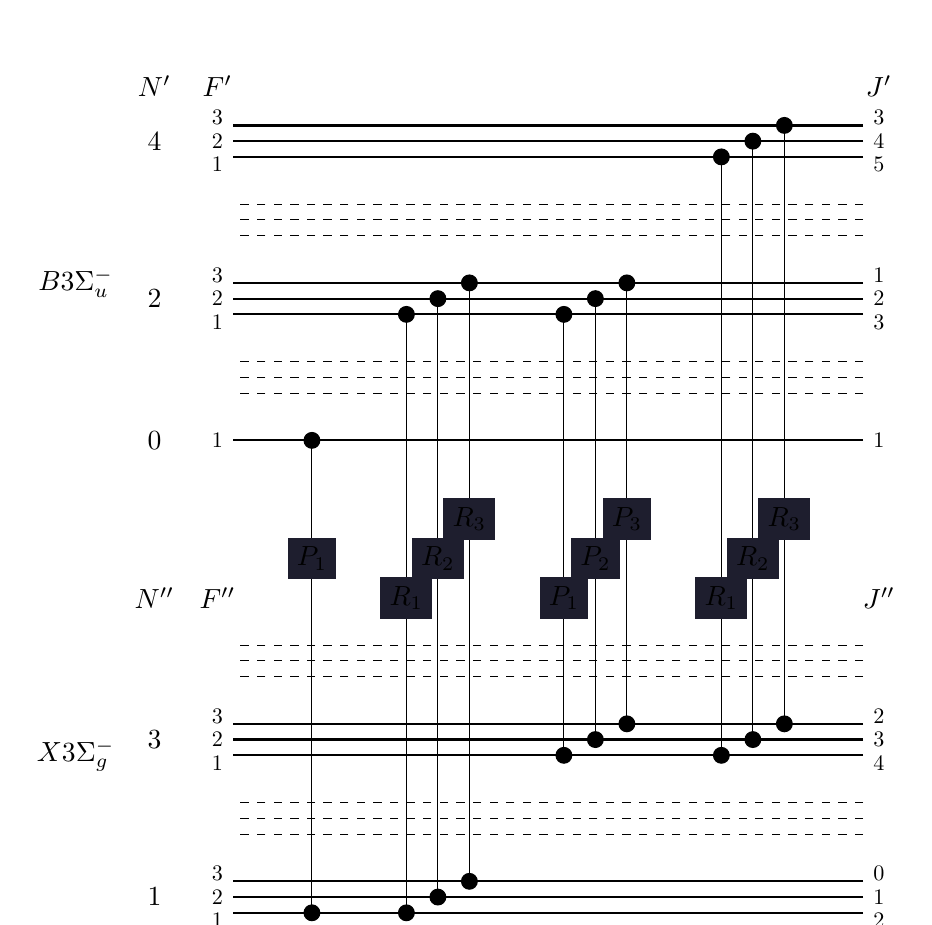
\begin{tikzpicture}
        \node at (-1,10.5) {$N'$};
        \node at (-0.2,10.5) {$F'$};
        \node at (8.2,10.5) {$J'$};

        \node at(-2,8) {$B\state{3}{\Sigma}_{u}^{-}$};

        \draw[thick] (8,10) -- (0,10);
        \node[scale=0.8] at (-0.2,10.1) {3};
        \node[scale=0.8] at (8.2,10.1) {3};
        \draw[thick] (8,9.8) -- (0,9.8);
        \node[scale=0.8] at (-0.2,9.8) {2};
        \node[scale=0.8] at (8.2,9.8) {4};
        \node at (-1,9.8) {4};
        \draw[thick] (8,9.6) -- (0,9.6);
        \node[scale=0.8] at (-0.2,9.5) {1};
        \node[scale=0.8] at (8.2,9.5) {5};

        \draw[dashed] (8,9) -- (0,9);
        \draw[dashed] (8,8.8) -- (0,8.8);
        \draw[dashed] (8,8.6) -- (0,8.6);

        \draw[thick] (8,8) -- (0,8);
        \node[scale=0.8] at (-0.2,8.1) {3};
        \node[scale=0.8] at (8.2,8.1) {1};
        \draw[thick] (8,7.8) -- (0,7.8);
        \node[scale=0.8] at (-0.2,7.8) {2};
        \node[scale=0.8] at (8.2,7.8) {2};
        \node at (-1,7.8) {2};
        \draw[thick] (8,7.6) -- (0,7.6);
        \node[scale=0.8] at (-0.2,7.5) {1};
        \node[scale=0.8] at (8.2,7.5) {3};

        \draw[dashed] (8,7) -- (0,7);
        \draw[dashed] (8,6.8) -- (0,6.8);
        \draw[dashed] (8,6.6) -- (0,6.6);

        \draw[thick] (8,6) -- (0,6);
        \node[scale=0.8] at (-0.2,6) {1};
        \node[scale=0.8] at (8.2,6) {1};
        \node at (-1,6) {0};

        \node at (-1,4) {$N''$};
        \node at (-0.2,4) {$F''$};
        \node at (8.2,4) {$J''$};

        \node at(-2,2) {$X\state{3}{\Sigma}_{g}^{-}$};

        \draw[dashed] (8,3.4) -- (0,3.4);
        \draw[dashed] (8,3.2) -- (0,3.2);
        \draw[dashed] (8,3) -- (0,3);

        \draw[thick] (8,2.4) -- (0,2.4);
        \node[scale=0.8] at (-0.2,2.5) {3};
        \node[scale=0.8] at (8.2,2.5) {2};
        \draw[thick] (8,2.2) -- (0,2.2);
        \node[scale=0.8] at (-0.2,2.2) {2};
        \node[scale=0.8] at (8.2,2.2) {3};
        \node at (-1,2.2) {3};
        \draw[thick] (8,2) -- (0,2);
        \node[scale=0.8] at (-0.2,1.9) {1};
        \node[scale=0.8] at (8.2,1.9) {4};

        \draw[dashed] (8,1.4) -- (0,1.4);
        \draw[dashed] (8,1.2) -- (0,1.2);
        \draw[dashed] (8,1) -- (0,1);

        \draw[thick] (8,0.4) -- (0,0.4);
        \node[scale=0.8] at (-0.2,0.5) {3};
        \node[scale=0.8] at (8.2,0.5) {0};
        \draw[thick] (8,0.2) -- (0,0.2);
        \node[scale=0.8] at (-0.2,0.2) {2};
        \node[scale=0.8] at (8.2,0.2) {1};
        \node at (-1,0.2) {1};
        \draw[thick] (8,0) -- (0,0);
        \node[scale=0.8] at (-0.2,-0.1) {1};
        \node[scale=0.8] at (8.2,-0.1) {2};

        \draw (1,6) -- (1,0);
        \filldraw (1,6) circle (0.1);
        \filldraw (1,0) circle (0.1);
        \node[fill=bgcolor] at (1,4.5) {$P_{1}$};

        \draw (2.2,7.6) -- (2.2,0);
        \filldraw (2.2,7.6) circle (0.1);
        \filldraw (2.2,0) circle (0.1);
        \node[fill=bgcolor] at (2.2,4) {$R_{1}$};
        \draw (2.6,7.8) -- (2.6,0.2);
        \filldraw (2.6,7.8) circle (0.1);
        \filldraw (2.6,0.2) circle (0.1);
        \node[fill=bgcolor] at (2.6,4.5) {$R_{2}$};
        \draw (3,8) -- (3,0.4);
        \filldraw (3,8) circle (0.1);
        \filldraw (3,0.4) circle (0.1);
        \node[fill=bgcolor] at (3,5) {$R_{3}$};

        \draw (4.2,7.6) -- (4.2,2);
        \filldraw (4.2,7.6) circle (0.1);
        \filldraw (4.2,2) circle (0.1);
        \node[fill=bgcolor] at (4.2,4) {$P_{1}$};
        \draw (4.6,7.8) -- (4.6,2.2);
        \filldraw (4.6,7.8) circle (0.1);
        \filldraw (4.6,2.2) circle (0.1);
        \node[fill=bgcolor] at (4.6,4.5) {$P_{2}$};
        \draw (5,8) -- (5,2.4);
        \filldraw (5,8) circle (0.1);
        \filldraw (5,2.4) circle (0.1);
        \node[fill=bgcolor] at (5,5) {$P_{3}$};

        \draw (6.2,9.6) -- (6.2,2);
        \filldraw (6.2,9.6) circle (0.1);
        \filldraw (6.2,2) circle (0.1);
        \node[fill=bgcolor] at (6.2,4) {$R_{1}$};
        \draw (6.6,9.8) -- (6.6,2.2);
        \filldraw (6.6,9.8) circle (0.1);
        \filldraw (6.6,2.2) circle (0.1);
        \node[fill=bgcolor] at (6.6,4.5) {$R_{2}$};
        \draw (7,10) -- (7,2.4);
        \filldraw (7,10) circle (0.1);
        \filldraw (7,2.4) circle (0.1);
        \node[fill=bgcolor] at (7,5) {$R_{3}$};
    \end{tikzpicture}
    \caption{Primary branch transitions between rotational levels of the Schumann--Runge system of molecular oxygen.}
\end{figure}

\begin{figure}[H]
    \centering
    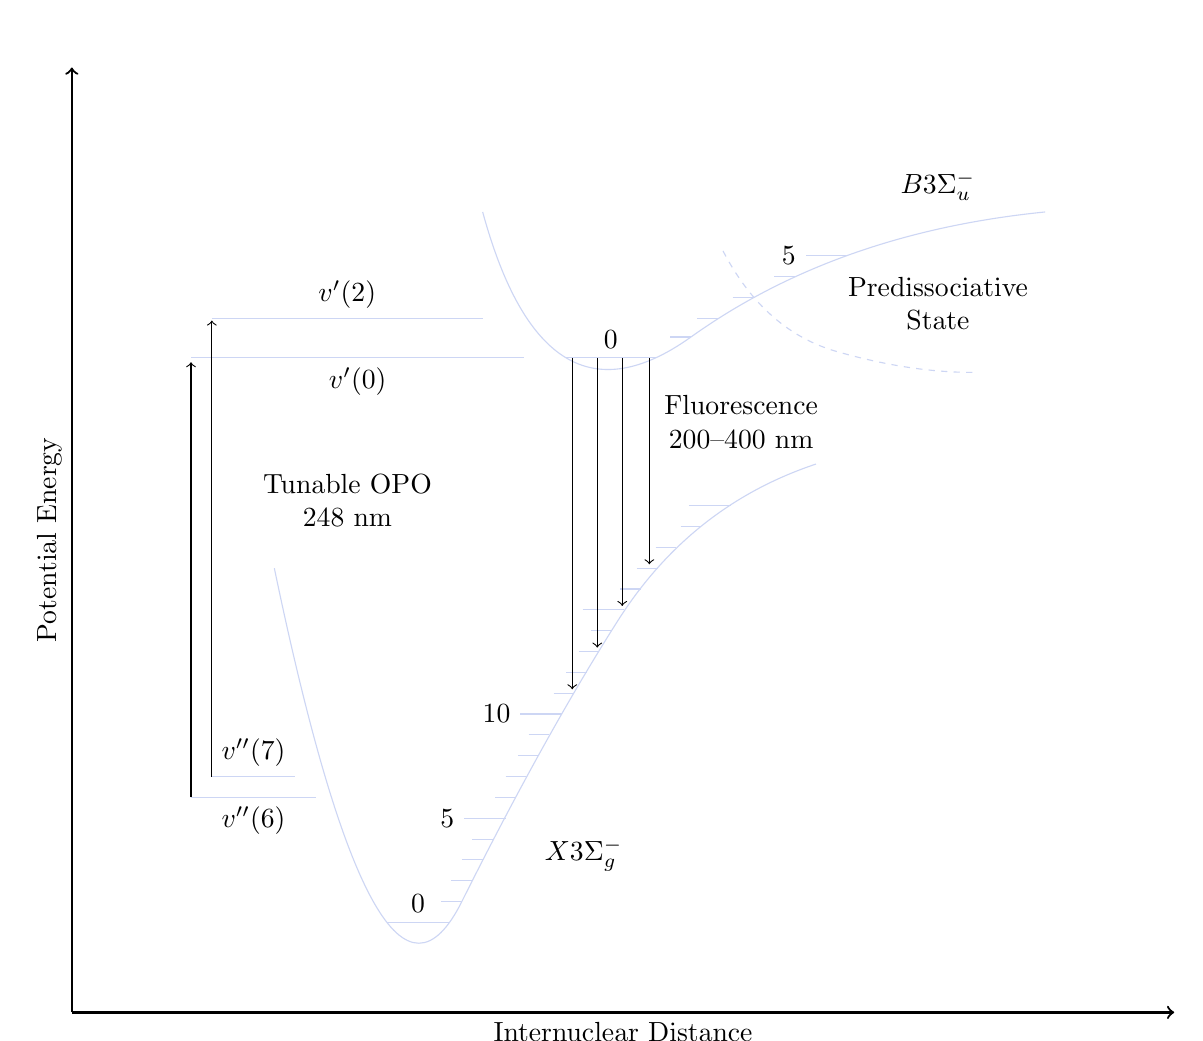
\begin{tikzpicture}
        % Excited state
        \path[draw=fgcolor] (6.2177, 11.1654) .. controls (6.7469, 9.2251) and (7.6288, 8.696) .. (8.8635, 9.5779) .. controls (10.0983, 10.4599) and (11.5976, 10.989) .. (13.3615, 11.1654);

        % Ground state
        \path[draw=fgcolor] (3.5719, 6.641) .. controls (4.4538, 2.4077) and (5.2476, 0.9966) .. (5.9531, 2.4077) .. controls (6.6587, 3.8188) and (7.3201, 5.0094) .. (7.9375, 5.9796) .. controls (8.5549, 6.9497) and (9.3927, 7.6112) .. (10.451, 7.964);

        % Predissociative state
        \path[draw=fgcolor,dash pattern=on 0.0794cm off 0.0794cm] (12.4354, 9.1281) .. controls (11.9063, 9.1281) and (11.333, 9.2163) .. (10.7156, 9.3927) .. controls (10.0983, 9.5691) and (9.6132, 10.0013) .. (9.2604, 10.6892);
        
        % Ground state energy levels
        \path[draw=fgcolor] (5.0006, 2.1431) -- (5.7944, 2.1431) node[midway,above] {$0$};
        \path[draw=fgcolor] (5.6885, 2.4077) -- (5.9531, 2.4077);
        \path[draw=fgcolor] (5.8208, 2.6723) -- (6.0854, 2.6723);
        \path[draw=fgcolor] (5.9531, 2.9369) -- (6.2177, 2.9369);
        \path[draw=fgcolor] (6.0854, 3.2015) -- (6.35, 3.2015);
        \path[draw=fgcolor] (6.5088, 3.466) -- (5.9796, 3.466) node[left] {$5$};
        \path[draw=fgcolor] (6.3765, 3.7306) -- (6.641, 3.7306);
        \path[draw=fgcolor] (6.5088, 3.9952) -- (6.7733, 3.9952);
        \path[draw=fgcolor] (6.6675, 4.2598) -- (6.9321, 4.2598);
        \path[draw=fgcolor] (6.7998, 4.5244) -- (7.0644, 4.5244);
        \path[draw=fgcolor] (7.2231, 4.789) -- (6.694, 4.789) node[left] {$10$};
        \path[draw=fgcolor] (7.1173, 5.0535) -- (7.3819, 5.0535);
        \path[draw=fgcolor] (7.276, 5.3181) -- (7.5406, 5.3181);
        \path[draw=fgcolor] (7.4348, 5.5827) -- (7.6994, 5.5827);
        \path[draw=fgcolor] (7.5935, 5.8473) -- (7.8581, 5.8473);
        \path[draw=fgcolor] (7.4877, 6.1119) -- (8.0169, 6.1119);
        \path[draw=fgcolor] (7.964, 6.3765) -- (8.2285, 6.3765);
        \path[draw=fgcolor] (8.1756, 6.641) -- (8.4402, 6.641);
        \path[draw=fgcolor] (8.4138, 6.9056) -- (8.6783, 6.9056);
        \path[draw=fgcolor] (8.7313, 7.1702) -- (8.9958, 7.1702);
        \path[draw=fgcolor] (8.8371, 7.4348) -- (9.3663, 7.4348);

        % Upper state energy levels
        \path[draw=fgcolor] (7.276, 9.3133) -- (8.4138, 9.3133) node[midway,above] {$0$};
        \path[draw=fgcolor] (8.599, 9.5779) -- (8.8635, 9.5779);
        \path[draw=fgcolor] (8.9429, 9.816) -- (9.2075, 9.816);
        \path[draw=fgcolor] (9.3927, 10.0806) -- (9.6573, 10.0806);
        \path[draw=fgcolor] (9.9219, 10.3452) -- (10.1865, 10.3452);
        \path[draw=fgcolor] (10.8479, 10.6098) -- (10.3188, 10.6098) node[left] {$5$};
        
        % Fluorescence lines
        \path[draw=fgcolor] (2.5135, 3.7306) -- (4.101, 3.7306) node[midway,below] {$v''(6)$};
        \path[draw=fgcolor] (2.7781, 3.9952) -- (3.8365, 3.9952) node[midway,above] {$v''(7)$};
        \path[draw=fgcolor] (2.5135, 9.3133) -- (6.7469, 9.3133) node[midway,below] {$v'(0)$};
        \path[draw=fgcolor] (2.7781, 9.816) -- (6.2177, 9.816) node[midway,above] {$v'(2)$};

        % Absorption arrows
        \draw[->] (2.5135, 3.7306) -- (2.5135, 9.2572);
        \draw[->] (2.7781, 3.9952) -- (2.7781, 9.7864);

        % Axes
        \draw[->,thick] (1, 1) -- (15, 1) node[midway,below] {Internuclear Distance};
        \draw[->,thick] (1, 1) -- (1, 13) node[midway,above,rotate=90] {Potential Energy};

        % Fluorescence arrows
        \draw[->] (7.3554, 9.3133) -- (7.3554, 5.1035);
        \draw[->] (7.6729, 9.3133) -- (7.6729, 5.6327);
        \draw[->] (7.9904, 9.3133) -- (7.9904, 6.1619);
        \draw[->] (8.3344, 9.3133) -- (8.3344, 6.691);

        % Labels
        \node at(7.5, 3) {$X\state{3}{\Sigma}_{g}^{-}$};
        \node at(12, 11.5) {$B\state{3}{\Sigma}_{u}^{-}$};
        \node[align=center] at(12, 10) {Predissociative\\State};
        \node[align=center] at(9.5, 8.5) {Fluorescence\\200--400 nm};
        \node[align=center] at(4.5, 7.5) {Tunable OPO\\248 nm};
    \end{tikzpicture}
    \caption{Potential energy diagram for the two electronic states of the Schumann--Runge band system.}
\end{figure}

\section{Total Energy}

 (Herzberg p. 149)
According to the Born--Oppenheimer approximation, the total energy of a molecule can be approximated as the sum of translational, electronic, vibrational, rotational, and nuclear components; that is
\begin{equation*}
    E = E_{t} + E_{e} + E_{v} + E_{r} + E_{n}.
\end{equation*}
In molecular spectroscopy, the components of interest are the electronic, vibrational, and rotational energies. Writing this equation using term values yields
\begin{equation*}
    T = T_{e} + G + F.
\end{equation*}
The wave numbers of the spectral lines corresponding to the transitions between two electronic states are given by
\begin{equation*}
    \nu = T' - T'' = (T_{e}' - T_{e}'') + (G' - G'') + (F' - F'').
\end{equation*}
This equation implies that the emitted or absorbed frequencies are composed of the electronic, vibrational, and rotational components:
\begin{equation*}
    \nu = \nu_{e} + \nu_{v} + \nu_{r}.
\end{equation*}

\section{Rotational Structure}

 (Herzberg p. 168)
For a specific vibrational transition, the quantity
\begin{equation*}
    \nu_{0} = \nu_{e} + \nu_{v},
\end{equation*}
called the band origin, is constant, while $\nu_{r}$ is variable and depends on the value of the rotational quantum numbers of the upper and lower states. Therefore, the wavenumbers of a rovibrational band can be computed as
\begin{equation*}
    \nu = \nu_{0} + F'(J') - F''(J'').
\end{equation*}

\section{Term Values}

 (Herzberg, p. 109)
The term values of the vibrating rotator can be expressed in the form of a double power series called the Dunham expansion, where
\begin{equation*}
    T = \sum_{lj}Y_{lj}\ab(v + \tfrac{1}{2})^{l} [J(J + 1)]^{j}.
\end{equation*}
(Babou, 2009)
The relations between Dunham coefficients $Y_{lj}$ and spectroscopic constants are shown below in \cref{t:dunham_coefficients}.
\begin{table}[H]
    \centering
    \caption{Relations between Dunham coefficients and spectroscopic constants.}
    \label{t:dunham_coefficients}
    \begin{tabular}{c|ccccc}
        \toprule
        $l$ & $j = 0$            & $j = 1$           & $j = 2$      & $j = 3$ & $j = 4$ \\
        \midrule
        0   & $Y_{00}$           & $B_{e}$           & $-D_{e}$     & $H_{e}$ & $L_{e}$ \\
        1   & $\omega_{e}$       & $-\alpha_{e}$     & $-\beta_{e}$ &         &         \\
        2   & $-\omega_{e}x_{e}$ & $\gamma_{e}$      & $-g_{e}$     &         &         \\
        3   & $\omega_{e}y_{e}$  & $\delta_{e}$      & $-h_{e}$     &         &         \\
        4   & $\omega_{e}z_{e}$  & $\varepsilon_{e}$ & $-k_{e}$     &         &         \\
        5   & $\omega_{e}a_{e}$  & $\xi_{e}$         &              &         &         \\
        6   & $\omega_{e}b_{e}$  & $\eta_{e}$        &              &         &         \\
        7   & $\omega_{e}c_{e}$  & $\theta_{e}$      &              &         &         \\
        8   & $\omega_{e}d_{e}$  &                   &              &         &         \\
        9   & $\omega_{e}e_{e}$  &                   &              &         &         \\
        \bottomrule
    \end{tabular}
\end{table}
(Herzberg p. 109)
The first coefficient represents the addition to the zero-point energy above that of the anharmonic oscillator, which is
\begin{equation*}
    Y_{00} = \frac{B_{e}}{4} + \frac{\alpha_{e}\omega_{e}}{12B_{e}} + \frac{\alpha_{e}^{2}\omega_{e}^{2}}{144B_{e}^{2}} - \omega_{e}x_{e}.
\end{equation*}

(Babou, 2009)
The vibrational term value can be expanded as a power series following the approach of Dunham, which yields
\begin{align*}
    G & = \omega_{e}\ab(v + \tfrac{1}{2}) - \omega_{e}x_{e}\ab(v + \tfrac{1}{2})^{2} + \omega_{e}y_{e}\ab(v + \tfrac{1}{2})^{3} + \omega_{e}z_{e}\ab(v + \tfrac{1}{2})^{4} + \omega_{e}a_{e}\ab(v + \tfrac{1}{2})^{5} \\
      & + \omega_{e}b_{e}\ab(v + \tfrac{1}{2})^{6} + \omega_{e}c_{e}\ab(v + \tfrac{1}{2})^{7} + \omega_{e}d_{e}\ab(v + \tfrac{1}{2})^{8} + \omega_{e}e_{e}\ab(v + \tfrac{1}{2})^{9} + \dotsb.
\end{align*}
Similarly, expansion of the rotational term value gives
\begin{equation*}
    F = B_{v}J(J + 1) - D_{v}[J(J + 1)]^{2} + H_{v}[J(J + 1)]^{3} + L_{v}[J(J + 1)]^{4} + \dotsb.
\end{equation*}
Note that the rotational expansion in particular is only a rough approximation and does not include the fine structure effects caused by spin-spin, spin-orbit, or spin-rotation coupling. These additions are made depending on the specific molecule under consideration. The rotational constants present within the rotational term value are expressed as
\begin{align*}
    B_{v} & = B_{e} - \alpha_{e}\ab(v + \tfrac{1}{2}) + \gamma_{e}\ab(v + \tfrac{1}{2})^{2} + \delta_{e}\ab(v + \tfrac{1}{2})^{3} + \varepsilon_{e}\ab(v + \tfrac{1}{2})^{4} + \xi_{e}\ab(v + \tfrac{1}{2})^{5} + \eta_{e}\ab(v + \tfrac{1}{2})^{6} \\
          & + \theta_{e}\ab(v + \tfrac{1}{2})^{7} + \dotsb,                                                                                                                                                                                         \\
    D_{v} & = D_{e} + \beta_{e}\ab(v + \tfrac{1}{2}) + g_{e}\ab(v + \tfrac{1}{2})^{2} + h_{e}\ab(v + \tfrac{1}{2})^{3} + k_{e}\ab(v + \tfrac{1}{2})^{4} + \dotsb,                                                                                   \\
    H_{v} & = H_{e} + \dotsb,
\end{align*}
and
\begin{equation*}
    L_{v} = L_{e} + \dotsb.
\end{equation*}

(Amiot 1981, Eq. 1)
The Hamiltonian for the $X\state{3}{\Sigma}_{g}^{-}$ ground state of \ce{O2} can be expressed as the sum of rotational, spin-spin, and spin-rotation interactions. Namely,
\begin{equation*}
    H = H_{r} + H_{ss} + H_{sr},
\end{equation*}
where
\begin{align*}
    H_{r}  & = B\vb{N}^{2} - D\vb{N}^{4},                    \\
    H_{ss} & = \tfrac{2}{3}\lambda(3S_{z}^{2} - \vb{S}^{2}),
\end{align*}
and
\begin{equation*}
    H_{sr} = \gamma\vb{N}\vdot\vb{S}.
\end{equation*}
The spin-spin and spin-rotation coupling constants, $\lambda$ and $\gamma$ respectively, can be written as
\begin{align*}
    \lambda & = \lambda_{0} + \lambda_{1}\vb{N}^{2} \\
    \gamma  & = \gamma_{0} + \gamma_{1}\vb{N}^{2}.
\end{align*}

(Amiot 1981, Eq. 1)
In a Hund's case (b) basis, the matrix representation of the three Hamiltonians for a given $J$ is
\begin{align*}
    H_{r}                                          & = B\bmx{
    J(J - 1)                                       & 0                                                        & 0                   \\
    0                                              & (J + 1)(J + 2)                                           & 0                   \\
    0                                              & 0                                                        & J(J + 1)
    }                                                                                                                               \\
                                                   & - D\bmx{
    J^{2}(J - 1)^{2}                               & 0                                                        & 0                   \\
    0                                              & (J + 1)^{2}(J + 2)^{2}                                   & 0                   \\
    0                                              & 0                                                        & J^{2}(J + 1)^{2}
    }                                                                                                                               \\
    H_{ss}                                         & = \lambda_{0}\bmx{
    \frac{2}{3} - \frac{2J}{2J + 1}                & \frac{2\sqrt{J(J + 1)}}{2J + 1}                          & 0                   \\
    \frac{2\sqrt{J(J + 1)}}{2J + 1}                & \frac{2}{3} - \frac{2(J + 1)}{2J + 1}                    & 0                   \\
    0                                              & 0                                                        & \frac{2}{3}
    }                                                                                                                               \\
                                                   & + \lambda_{1}\bmx{
    \ab(\frac{2}{3} - \frac{2J}{2J + 1})J(J - 1)   & \frac{2\sqrt{J(J + 1)}}{2J + 1}(J^{2} + J + 1)           & 0                   \\
    \frac{2\sqrt{J(J + 1)}}{2J + 1}(J^{2} + J + 1) & \ab(\frac{2}{3} - \frac{2(J + 1)}{2J + 1})(J + 1)(J + 2) & 0                   \\
    0                                              & 0                                                        & \frac{2}{3}J(J + 1)
    }                                                                                                                               \\
    H_{sr}                                         & = \gamma_{0}\bmx{
    J - 1                                          & 0                                                        & 0                   \\
    0                                              & -(J + 2)                                                 & 0                   \\
    0                                              & 0                                                        & -1
    }
    + \gamma_{1}\bmx{
    J(J - 1)^{2}                                   & 0                                                        & 0                   \\
    0                                              & -(J + 2)^{2}(J + 1)                                      & 0                   \\
    0                                              & 0                                                        & -J(J + 1)
    }.
\end{align*}

(Cheung, 1986) Using the same Hamiltonian, the combined matrix elements in a Hund's case (a) basis can also be written as
\begin{align*}
    F_{2}      & = T + Bx - Dx^{2} + \tfrac{2}{3}\lambda - \gamma + \tfrac{2}{3}\lambda_{D}x - \gamma_{D}x, \\
    F_{1}F_{3} & = \bmx{
    H_{11}     & H_{12}                                                                                     \\ H_{21} & H_{22}
    },
\end{align*}
where
\begin{align*}
    H_{11} & = T + B(x + 2) - D(x^{2} + 8x + 4) - \tfrac{4}{3}\lambda - 2\gamma - \tfrac{4}{3}\lambda_{D}(x + 2) - 4\gamma_{D}(x + 1) \\
    H_{12} & = -2\sqrt{x}\ab[B - 2D(x + 1) - \tfrac{\gamma}{2} - \tfrac{2}{3}\lambda_{D} - \tfrac{1}{2}\gamma_{D}(x + 4)]             \\
    H_{21} & = H_{12}                                                                                                                 \\
    H_{22} & = T + Bx - D(x^{2} + 4x) + \tfrac{2}{3}\lambda - \gamma + \tfrac{2}{3}x\lambda_{D} - 3x\gamma_{D}.
\end{align*}
Note that
\begin{equation*}
    x = J(J + 1).
\end{equation*}

\section{Main and Satellite Branches}

 (Herzberg p. 249) The six main branches in $\state{3}{\Sigma}\dash\state{3}{\Sigma}$ transitions are
\begin{align*}
    P_{1} & = \nu_{0} + F'_{1}(J - 1) - F''_{1}(J)  \\
    R_{1} & = \nu_{0} + F'_{1}(J + 1) - F''_{1}(J)  \\
    P_{2} & = \nu_{0} + F'_{2}(J - 1) - F''_{2}(J)  \\
    R_{2} & = \nu_{0} + F'_{2}(J + 1) - F''_{2}(J)  \\
    P_{3} & = \nu_{0} + F'_{3}(J - 1) - F''_{3}(J)  \\
    R_{3} & = \nu_{0} + F'_{3}(J + 1) - F''_{3}(J).
\end{align*}
The six satellite branches are
\begin{align*}
    \state{P}{Q}_{12} & = \nu_{0} + F'_{1}(J - 1) - F''_{2}(J)  \\
    \state{R}{Q}_{21} & = \nu_{0} + F'_{2}(J + 1) - F''_{1}(J)  \\
    \state{P}{Q}_{13} & = \nu_{0} + F'_{1}(J - 1) - F''_{3}(J)  \\
    \state{R}{Q}_{31} & = \nu_{0} + F'_{3}(J + 1) - F''_{1}(J)  \\
    \state{P}{Q}_{23} & = \nu_{0} + F'_{2}(J - 1) - F''_{3}(J)  \\
    \state{R}{Q}_{32} & = \nu_{0} + F'_{3}(J + 1) - F''_{2}(J).
\end{align*}

\section{H\"onl--London Factors}

 (Tatum, 1966)
The rotational line strength factors for $\state{3}{\Sigma}^{\pm}\dash\state{3}{\Sigma}^{\pm}$ transitions are shown below in \cref{t:honl_london_factors_3s}.
\begin{table}[H]
    \centering
    \caption{H\"onl--London Factors for $\state{3}{\Sigma}^{\pm}\dash\state{3}{\Sigma}^{\pm}$ transitions.}
    \label{t:honl_london_factors_3s}
    \begin{tabular}{ccc}
        \toprule
        Branch              & Emission                                & Absorption                                 \\
        \midrule
        $P_{1}$             & $\dfrac{(N' + 1)(2N' + 5)}{2N' + 3}$    & $\dfrac{N''(2N'' + 3)}{2N'' + 1}$          \\
        \addlinespace[0.5em]
        $R_{1}$             & $\dfrac{N'(2N' + 3)}{2N' + 1}$          & $\dfrac{(N'' + 1)(2N'' + 5)}{2N'' + 3}$    \\
        \addlinespace[0.5em]
        $\state{P}{Q}_{13}$ & $\dfrac{1}{(N' + 1)(2N' + 1)(2N' + 3)}$ & $\dfrac{1}{N''(2N'' - 1)(2N'' + 1)}$       \\
        \addlinespace[0.5em]
        $\state{P}{Q}_{12}$ & $\dfrac{1}{N' + 1}$                     & $\dfrac{1}{N''}$                           \\
        \addlinespace[0.5em]
        $P_{2}$             & $\dfrac{N'(N' + 2)}{N' + 1}$            & $\dfrac{(N'' - 1)(N'' + 1)}{N''}$          \\
        \addlinespace[0.5em]
        $R_{2}$             & $\dfrac{(N' - 1)(N' + 1)}{N'}$          & $\dfrac{N''(N'' + 2)}{N'' + 1}$            \\
        \addlinespace[0.5em]
        $\state{P}{Q}_{23}$ & $\dfrac{1}{N' + 1}$                     & $\dfrac{1}{N''}$                           \\
        \addlinespace[0.5em]
        $\state{R}{Q}_{21}$ & $\dfrac{1}{N'}$                         & $\dfrac{1}{N'' + 1}$                       \\
        \addlinespace[0.5em]
        $P_{3}$             & $\dfrac{(N' + 1)(2N' - 1)}{2N' + 1}$    & $\dfrac{N''(2N'' - 3)}{2N'' - 1}$          \\
        \addlinespace[0.5em]
        $R_{3}$             & $\dfrac{N'(2N' - 3)}{2N' - 1}$          & $\dfrac{(N'' + 1)(2N'' - 1)}{2N'' + 1}$    \\
        \addlinespace[0.5em]
        $\state{R}{Q}_{32}$ & $\dfrac{1}{N'}$                         & $\dfrac{1}{N'' + 1}$                       \\
        \addlinespace[0.5em]
        $\state{R}{Q}_{31}$ & $\dfrac{1}{N'(2N' - 1)(2N' + 1)}$       & $\dfrac{1}{(N'' + 1)(2N'' + 1)(2N'' + 3)}$ \\
        \bottomrule
    \end{tabular}
\end{table}

\section{Spectral Lineshapes}

\subsection{Lorentzian Profile}

From \textit{A Student's Guide to Atomic Physics} by Fox, Eq. (3.31) and \textit{Spectroscopy and Optical Diagnostics for Gases} by Hanson, Eq. (8.7):
\begin{equation*}
    \phi_{L}(\nu) = \frac{1}{2\pi}\frac{\adif{\nu}}{(\nu - \nu_{0})^{2} + (\adif{\nu}/2)^{2}}
\end{equation*}

From \textit{A Student's Guide to Atomic Physics} by Fox, Eq. (3.32) and \textit{Spectroscopy and Optical Diagnostics for Gases} by Hanson, Eq. (8.6):
\begin{equation*}
    \adif{\nu} = \frac{1}{2\pi}\ab(\frac{1}{\tau'} + \frac{1}{\tau''})
\end{equation*}

\subsection{Natural Broadening}

The lifetime of an atom in a particular level is determined by spontaneous emission, which is described by (Hanson, Eq. 8.11)
\begin{equation*}
    \adif{\nu}_{N} = \frac{1}{2\pi}\ab(\sum_{k} A_{ik} + \sum_{k} A_{jk}).
\end{equation*}
This represents the sum of the Einstein $A$ coefficients for all downward transitions from the two levels of the transitions $i$ and $j$. The sum is therefore over all $k$ such that $E_{k} < E_{i}$ or $E_{k} < E_{j}$. If the lower level $j$ is the ground state, there can be no radiative decay and its contribution to the FWHM is zero.

\paragraph{Unit Verification}

The units of $\adif{\nu}_{N}$ using the formula given are inverse seconds, as shown by the following:
\begin{equation*}
    \adif{\nu}_{N} = \unit{s^{-1}}.
\end{equation*}
To convert to wavenumbers in $\unit{cm^{-1}}$, divide by the speed of light in $\unit{cm/s}$.

\subsection{Collisional Broadening}

The collisional cross-section between two molecules is given as (Hanson, Eq. 8.12 and Plasma Physics Slideset 5, page 5)
\begin{equation*}
    \sigma_{AB} = \pi d_{AB}^{2} = \pi\ab(\frac{d_{A} + d_{B}}{2})^{2},
\end{equation*}
where $d_{AB}$ is the optical collision diameter of the two molecules. Following this, the number of collisions per second of a single molecule $B$ with all $A$ is (Hanson Eq. 8.13)
\begin{equation*}
    Z_{AB} = n_{A}\sigma_{AB}\bar{v},
\end{equation*}
where $\bar{v}$ is the mean speed of the molecules and is given by (Hanson, Eq. 8.14)
\begin{equation*}
    \bar{v} = \sqrt{\frac{8kT}{\pi\mu_{AB}}}.
\end{equation*}
Here, $\mu_{AB}$ is the reduced mass of the two molecules, given by (Hanson, Eq. 8.15)
\begin{equation*}
    \mu_{AB} = \frac{m_{A}m_{B}}{m_{A} + m_{B}}.
\end{equation*}
The total collision frequency of a single $B$ is (Hanson Eq. 8.16)
\begin{equation*}
    Z_{B} = \sum_{A}N_{A}\sigma_{AB}\sqrt{\frac{8kT}{\pi\mu_{AB}}}.
\end{equation*}
Using the ideal gas law $p = NkT$, this expression becomes (Hanson Eq. 8.17)
\begin{equation*}
    Z_{B} = p\sum_{A}X_{A}\sigma_{AB}\sqrt{\frac{8}{\pi\mu_{AB}kT}},
\end{equation*}
where $X_{A}$ is the mole fraction of species $A$. If we assume that
\begin{equation*}
    \frac{1}{\tau'} = \frac{1}{\tau''} = Z_{B},
\end{equation*}
the FWHM due to collisional broadening is (Hanson Eq. 8.18)
\begin{equation*}
    \adif{\nu}_{C} = \frac{Z_{B}}{\pi}.
\end{equation*}
For a single species, this becomes
\begin{equation*}
    \adif{\nu}_{C} = \frac{p\sigma_{BB}}{\pi}\sqrt{\frac{8}{\pi\mu_{BB}kT}}.
\end{equation*}
The collisional cross-section for a single species mixture is
\begin{equation*}
    \sigma_{BB} = \pi\ab(\frac{d_{B} + d_{B}}{2})^{2} = \pi d_{B}^{2}.
\end{equation*}
The reduced mass for a single species mixture is
\begin{equation*}
    \mu_{BB} = \frac{m_{B}m_{B}}{m_{B} + m_{B}} = \frac{m_{B}^{2}}{2m_{B}} = \frac{m_{B}}{2}.
\end{equation*}

\paragraph{Unit Verification}

The units of $\adif{\nu}_{C}$ using the formula given are inverse seconds, as shown by the following:
\begin{equation*}
    \adif{\nu}_{C} = \unit{Pa.m^{2}}\sqrt{\frac{\unit{K}}{\unit{kg.J.K}}} = \unit{N}\sqrt{\frac{\unit{s^{2}}}{\unit{kg^{2}.m^{2}}}} = \frac{\unit{kg.m}}{\unit{s^{2}}}\frac{\unit{s}}{\unit{kg.m}} = \unit{s^{-1}}.
\end{equation*}
To convert to wavenumbers in $\unit{cm^{-1}}$, divide by the speed of light in $\unit{cm/s}$.

\subsection{Gaussian Profile}

From \textit{A Student's Guide to Atomic Physics} by Fox, Eq. (3.42) and \textit{Spectroscopy and Optical Diagnostics for Gases} by Hanson, Eq. (8.22):
\begin{equation*}
    \phi_{G}(\nu) = \frac{2}{\adif{\nu}}\sqrt{\frac{\ln{2}}{\pi}}\exp\ab[-4\ln{2}\ab(\frac{\nu - \nu_{0}}{\adif{\nu}})^{2}]
\end{equation*}

\subsection{Doppler Broadening}

From \textit{A Student's Guide to Atomic Physics} by Fox, Eq. (3.43) and \textit{Spectroscopy and Optical Diagnostics for Gases} by Hanson, Eq. (8.24):
\begin{equation*}
    \adif{\nu}_{D} = \nu_{0}\sqrt{\frac{8kT\ln{2}}{mc^{2}}}
\end{equation*}

\paragraph{Unit Verification}

The units of $\adif{\nu}_{D}$ using the formula given are inverse centimeters, as shown by the following:
\begin{equation*}
    \adif{\nu}_{D} = \unit{cm^{-1}}\sqrt{\frac{\unit{J.K.s^{2}}}{\unit{K.kg.m^{2}}}} = \unit{cm^{-1}}\sqrt{\frac{\unit{kg.m^{2}.s^{2}}}{\unit{kg.m^{2}.s^{2}}}} = \unit{cm^{-1}}.
\end{equation*}

\section{Transition Intensities}

The general formulae for spectral line intensities are given in Herzberg p. 20.
\begin{align*}
    I_{nm} & = N_{n}hc\nu_{nm}A_{nm}                  \\
    I_{nm} & = \rho_{nm}N_{m}hc\nu_{nm}B_{mn}\adif{x}
\end{align*}

\subsection{Einstein Coefficients}

The Einstein transition probability of spontaneous emission is
\begin{equation*}
    A_{nm} = \frac{64\pi^{4}\nu_{nm}^{3}}{3h}\abs{\vb{R}_{nm}}^{2}.
\end{equation*}
Similarly, the Einstein transition probability of absorption is
\begin{equation*}
    B_{mn} = \frac{8\pi^{3}}{3h^{2}c}\abs{\vb{R}_{nm}}^{2}.
\end{equation*}
These two equations are related by
\begin{equation*}
    B_{mn} = \frac{1}{8\pi hc\nu_{nm}^{3}}A_{nm}
\end{equation*}

For transitions between degenerate levels, the above formulae must be modified as such:
\begin{align*}
    A_{nm} & = \frac{64\pi^{4}\nu_{nm}^{3}}{3h}\frac{\sum\abs{\vb{R}_{n_{i}m_{i}}}^{2}}{d_{n}} \\
    B_{mn} & = \frac{8\pi^{3}}{3h^{2}c}\frac{\sum\abs{\vb{R}_{n_{i}m_{i}}}^{2}}{d_{m}}         \\
    B_{mn} & = \frac{1}{8\pi hc\nu_{nm}^{3}}\frac{d_{n}}{d_{m}}A_{nm}
\end{align*}

\subsection{Transition Moment}

From Herzberg, Eq. (IV, 67):
\begin{equation*}
    \vb{R} = \int \psi'\vb{M}\psi'' \odif{\tau}
\end{equation*}
From Herzberg, Eq. (VI, 58): (non-degenerate only?)
\begin{equation*}
    \vb{R} = \vb{R}_{e}^{nm}\vb{R}_{v}^{v'v''}\vb{R}_{r}^{J'J''}
\end{equation*}
The transition probability for absorption is given by Herzberg p. 382 as
\begin{equation*}
    B_{evr} = \frac{8\pi^{3}}{3h^{2}c}\frac{\sum\abs{\vb{R}}^{2}}{2J'' + 1} = \frac{8\pi^{3}}{3h^{2}c}\abs{\vb{R}_{e}}^{2}\abs{\vb{R}_{v}}^{2}\frac{\sum\abs{\vb{R}_{r}}^{2}}{2J'' + 1},
\end{equation*}
where
\begin{equation*}
    \abs{\vb{R}_{v}}^{2} = q_{v},
\end{equation*}
and
\begin{equation*}
    \abs{\vb{R}_{r}}^{2} = S_{J}.
\end{equation*}
Using these two substitutions,
\begin{equation*}
    B_{evr} = B_{e}q_{v}\frac{S_{J}}{2J'' + 1}.
\end{equation*}

\section{Partition Functions}

\subsection{General Form}

General form of the Boltzmann population distribution Hanson Eq. (1.11):
\begin{equation*}
    \frac{N_{i}}{N} = \frac{g_{i}}{Q}\exp\ab(-\frac{\varepsilon_{i}}{kT})
\end{equation*}
General form of the partition function Hanson Eq. (1.12):
\begin{equation*}
    Q = \sum_{i} g_{i}\exp\ab(-\frac{\varepsilon_{i}}{kT})
\end{equation*}
The total molecular partition function can be expressed as the product of the individual translational, electronic, vibrational, rotational, and nuclear components for symmetric molecules Hanson Eq. (5.4):
\begin{equation*}
    Q = Q_{t}Q_{e}Q_{v}Q_{r}Q_{n}
\end{equation*}

\subsection{Nuclear}

Nuclear partition function for a molecule Hanson Eq. (5.9):
\begin{equation*}
    Q_{n} = \prod_{i = 1}^{L} (2I_{n} + 1)
\end{equation*}

\subsection{Rotational}
Because of the rotational symmetry of certain molecules, a symmetry parameter $\sigma$ must be added to the rotational partition function to account for the multiple molecular orientations that are indistinguishable.
Herzberg Eq. (III, 164):
\begin{equation*}
    Q_{r} = \frac{1}{\sigma} \sum g_{r}\exp\ab(-\frac{\varepsilon_{r}}{kT})
\end{equation*}
The degeneracy of each state is
\begin{equation*}
    g_{r} = 2J + 1
\end{equation*}
and the rotational energy can be expressed as the term value
\begin{equation*}
    \varepsilon_{r} = F(J)hc.
\end{equation*}
Therefore, the rotational partition function is
\begin{equation*}
    Q_{r} = \frac{1}{\sigma} \sum (2J + 1)\exp\ab(-\frac{F(J)hc}{kT}).
\end{equation*}
For sufficiently large $T$ or small $B$,
Rotational partition function for a molecule in the high-temperature limit Hanson Eq. (2.21) and Herzberg Eq. (III, 166):
\begin{equation*}
    Q_{r} \approx \frac{1}{\sigma} \int_{0}^{\infty} (2J + 1)\exp\ab(-\frac{BJ(J + 1)hc}{kT}) \odif{J} = \frac{1}{\sigma}\frac{kT}{hcB}
\end{equation*}
The Boltzmann fraction is then
\begin{equation*}
    \frac{N_{J}}{N} = \frac{(2J + 1)}{Q_{r}}\exp\ab(-\frac{F(J)hc}{kT})
\end{equation*}

\subsection{Effective Rotational}

The effective rotational partition function for symmetric molecules is Hanson Eq. (5.5):
\begin{equation*}
    Q'_{r} = Q_{r}Q_{n}
\end{equation*}
Similarly, the effective rotational degeneracy is Hanson Eq. (5.6):
\begin{equation*}
    g'_{r} = g_{r}g_{n}
\end{equation*}
For homonuclear diatomic molecules, the effective rotational degeneracy is Hanson Eq. (5.16)
\begin{equation*}
    g'_{rot} = \frac{(2J + 1)}{2}\ab[(2I + 1)^{2} \pm (2I + 1)]
\end{equation*}

\subsection{Vibrational}

Herzberg Eq. (III, 159)
\begin{equation*}
    Q_{v} = \sum g_{v}\exp\ab(-\frac{\varepsilon_{v}}{kT})
\end{equation*}
The vibrational degeneracy of each state is
\begin{equation*}
    g_{v} = 1,
\end{equation*}
and the vibrational energy can be expressed as the term value
\begin{equation*}
    \varepsilon_{v} = G(v)hc.
\end{equation*}
Therefore, the vibrational partition function is
\begin{equation*}
    Q_{v} = \sum \exp\ab(-\frac{G(v)hc}{kT}).
\end{equation*}
The Boltzmann fraction is then
\begin{equation*}
    \frac{N_{v}}{N} = \frac{1}{Q_{v}}\exp\ab(-\frac{G(v)hc}{kT})
\end{equation*}
The vibrational partition function can also be written in terms of the zero-point vibrational energy as
\begin{equation*}
    Q_{v} = \sum \exp\ab(-\frac{[G(v) - G(0)]hc}{kT}).
\end{equation*}
The Boltzmann fraction is therefore
\begin{equation*}
    \frac{N_{v}}{N} = \frac{1}{Q_{v}}\exp\ab(-\frac{[G(v) - G(0)]hc}{kT}).
\end{equation*}

\subsection{Electronic}

Anderson Eq. (11.56)
\begin{equation*}
    Q_{e} = \sum g_{e}\exp\ab(-\frac{\varepsilon}{kT})
\end{equation*}
The electronic degeneracy depends on the individual states. The electronic energy can be expressed as the term value
\begin{equation*}
    \varepsilon_{e} = T_{e}hc.
\end{equation*}
Therefore, the electronic partition function is
\begin{equation*}
    Q_{e} = \sum g_{e}\exp\ab(-\frac{T_{e}hc}{kT}).
\end{equation*}
The Boltzmann fraction is therefore
\begin{equation*}
    \frac{N_{e}}{N} = \frac{g_{e}}{Q_{e}}\exp\ab(-\frac{T_{e}hc}{kT}).
\end{equation*}

\subsection{Translational}

Anderson Eq. (11.53)
\begin{equation*}
    Q_{t} = \ab(\frac{2\pi mkT}{h^{2}})^{3/2}V,
\end{equation*}
where $V$ is the volume of the system.

\section{Rate Equations}

\begin{figure}[H]
    \centering
    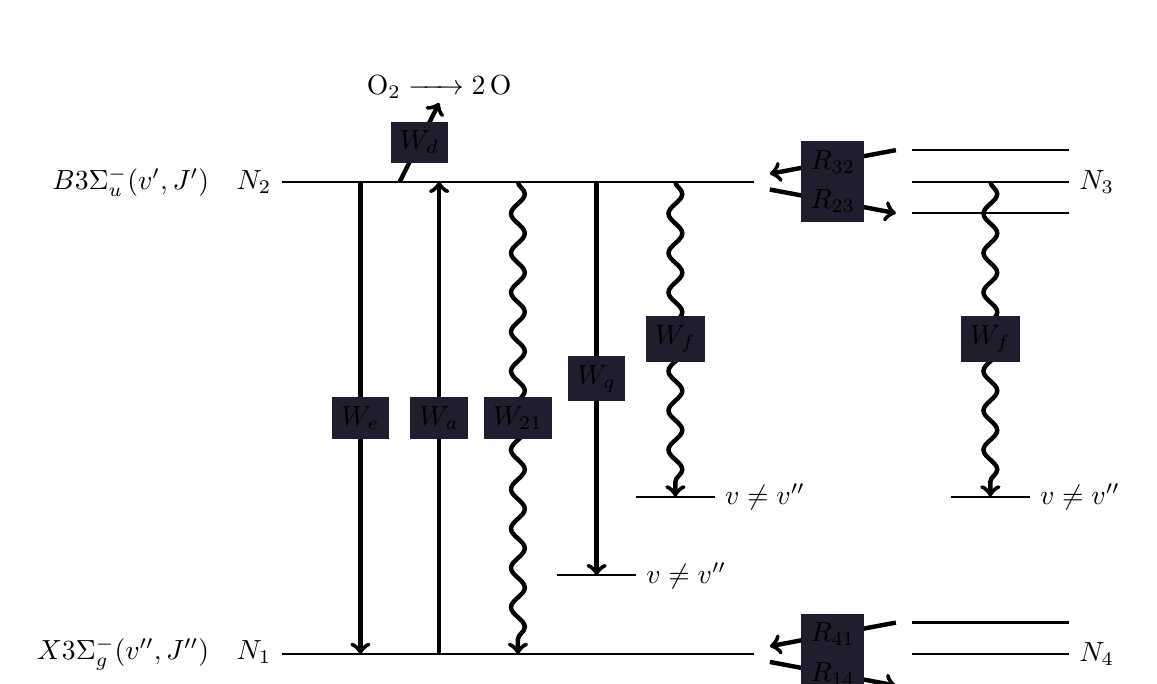
\begin{tikzpicture}
        \draw[thick] (6,0) -- (0,0) node[left] {$X\state{3}{\Sigma}_{g}^{-}(v'', J'') \quad N_{1}$};
        \draw[thick] (6,6) -- (0,6) node[left] {$B\state{3}{\Sigma}_{u}^{-}(v', J') \quad N_{2}$};

        \draw[->,ultra thick] (1,6) -- (1,0) node[midway,fill=bgcolor] {$W_{e}$};
        \draw[->,ultra thick] (1.5,6) -- (2,7) node[midway,fill=bgcolor] {$W_{d}$};
        \node at(2,7.2) {\ce{O2 -> 2O}};
        \draw[->,ultra thick] (2,0) -- (2,6) node[midway,fill=bgcolor] {$W_{a}$};
        \draw[->,ultra thick,decorate,decoration={snake,segment length=5mm}] (3,6) -- (3,0) node[midway,fill=bgcolor] {$W_{21}$};
        \draw[->,ultra thick] (4,6) -- (4,1) node[midway,fill=bgcolor] {$W_{q}$};
        \draw[thick] (3.5,1) -- (4.5,1) node[right] {$v \neq v''$};
        \draw[->,ultra thick,decorate,decoration={snake, segment length=5mm}] (5,6) -- (5,2) node[midway,fill=bgcolor] {$W_{f}$};
        \draw[thick] (4.5,2) -- (5.5,2) node[right] {$v \neq v''$};

        \draw[<-,ultra thick] (6.2,6.1) -- (7.8,6.4) node[midway,fill=bgcolor] {$R_{32}$};
        \draw[thick] (8,6.4) -- (10,6.4);
        \draw[thick] (8,6) -- (10,6) node[right] {$N_{3}$};
        \draw[thick] (8,5.6) -- (10,5.6);
        \draw[->,ultra thick] (6.2,5.9) -- (7.8,5.6) node[midway,fill=bgcolor] {$R_{23}$};

        \draw[->,ultra thick,decorate,decoration={snake,segment length=5mm}] (9,6) -- (9,2) node[midway,fill=bgcolor] {$W_{f}$};
        \draw[thick] (8.5,2) -- (9.5,2) node[right] {$v \neq v''$};

        \draw[<-,ultra thick] (6.2,0.1) -- (7.8,0.4) node[midway,fill=bgcolor] {$R_{41}$};
        \draw[thick] (8,0.4) -- (10,0.4);
        \draw[thick] (8,0) -- (10,0) node[right] {$N_{4}$};
        \draw[thick] (8,-0.4) -- (10,-0.4);
        \draw[->,ultra thick] (6.2,-0.1) -- (7.8,-0.4) node[midway,fill=bgcolor] {$R_{14}$};
    \end{tikzpicture}
    \caption{Four-level LIF model for the Schumann--Runge bands of molecular oxygen.}
\end{figure}

\subsection{Four-level LIF}

Grinstead thesis, Eq. (2.9)
\begin{align*}
    \odv{N_{1}}{t} & = -(W_{a} + R_{14})N_{1} + (W_{e} + W_{21})N_{2} + R_{41}N_{4}                      \\
    \odv{N_{2}}{t} & = W_{a}N_{1} - (W_{f} + W_{d} + W_{q} + W_{e} + W_{21} + R_{23})N_{2} + R_{32}N_{3} \\
    \odv{N_{3}}{t} & = R_{23}N_{2} - (W_{f} + R_{32})N_{3}                                               \\
    \odv{N_{4}}{t} & = R_{14}N_{1} - R_{41}N_{4}
\end{align*}
$W_{a}$ is the laser-stimulated absorption rate, $W_{e}$ the laser-stimulated emission rate, $W_{21}$ the spontaneous emission rate, $W_{d}$ the predissociation rate, $W_{q}$ the collisional quenching rate, $W_{f}$ the fluorescent radiative decay rate, and $R_{ij}$ the rotational energy transfer rates.

\subsection{Three-level LIF}

Diskin, 1996 Eqs. (1-3)
\begin{align*}
    \odv{N_{1}}{t} & = -W_{a}N_{1} + (W_{e} + W_{21})N_{2} + W_{c}\ab(\frac{f_{b}}{1 - f_{b}}N_{3} - N_{1}) \\
    \odv{N_{2}}{t} & = W_{a}N_{1} - (W_{e} + W_{d} + W_{21} + W_{f} + W_{q})N_{2}                           \\
    \odv{N_{3}}{t} & = -W_{c}\ab(\frac{f_{b}}{1 - f_{b}}N_{3} - N_{1})
\end{align*}

\appendix
\chapter{Diatomic Constants}
\label{a:diatomic_constants}

\begin{table}[H]
    \centering
    \caption{Diatomic constants for \ce{^{16}O2} \cite{nist:diatomic}.}
    \label{t:diatomic_constants_for_o2}
    \begin{tabular}{cccc}
        \toprule
        Symbol            & \multicolumn{2}{c}{State}    & Units                                           \\
        \cmidrule(lr){2-3}
                          & $X\state{3}{\Sigma}_{g}^{-}$ & $B\state{3}{\Sigma}_{u}^{-}$ &                  \\
        \midrule
        \multicolumn{4}{c}{\textit{Electronic}}                                                            \\
        \cmidrule(lr){1-4}
        $T_{e}$           & \num{0}                      & \num{49793.28}               & \unit{cm^{-1}}   \\
        \multicolumn{4}{c}{\textit{Vibrational}}                                                           \\
        \cmidrule(lr){1-4}
        $\omega_{e}$      & \num{1580.19(3)}             & \num{709.31}                 & \unit{cm^{-1}}   \\
        $\omega_{e}x_{e}$ & \num{11.98(1)}               & \num{10.65}                  & \unit{cm^{-1}}   \\
        $\omega_{e}y_{e}$ & \num{0.0474(7)}              & \num{-0.139}                 & \unit{cm^{-1}}   \\
        $\omega_{e}z_{e}$ & \num{-0.00127(3)}            &                              & \unit{cm^{-1}}   \\
        \multicolumn{4}{c}{\textit{Rotational}}                                                            \\
        \cmidrule(lr){1-4}
        $B_{e}$           & \num{1.4376766}              & \num{0.8190(2)}              & \unit{cm^{-1}}   \\
        $\alpha_{e}$      & \num{0.0159(3)}              & \num{0.01206}                & \unit{cm^{-1}}   \\
        $\gamma_{e}$      &                              & \num{-5.5(6)e-4}             & \unit{cm^{-1}}   \\
        $\delta_{e}$      &                              &                              & \unit{cm^{-1}}   \\
        \multicolumn{4}{c}{\textit{Centrifugal Distortion}}                                                \\
        \cmidrule(lr){1-4}
        $D_{e}$           &                              &                              & \unit{cm^{-1}}   \\
        $\beta_{e}$       &                              &                              & \unit{cm^{-1}}   \\
        \multicolumn{4}{c}{\textit{Spin-Splitting}}                                                        \\
        \cmidrule(lr){1-4}
        $\lambda$         &                              &                              & \unit{cm^{-1}}   \\
        $\gamma$          &                              &                              & \unit{cm^{-1}}   \\
        \multicolumn{4}{c}{\textit{Other}}                                                                 \\
        \cmidrule(lr){1-4}
        $H_{e}$           &                              &                              & \unit{cm^{-1}}   \\
        $r_{e}$           &                              &                              & \unit{\angstrom} \\
        $\nu_{00}$        &                              &                              & \unit{cm^{-1}}   \\
        \bottomrule
    \end{tabular}
\end{table}

\chapter{Notation for Diatomic Constants}
\label{a:notation_for_diatomic_constants}

\begin{table}[H]
    \centering
    \caption{Notation for diatomic constants \cite{herzberg:diatomic,nist:sigma1,nist:sigma3}.}
    \label{t:notation}
    \begin{tabular}{clc}
        \toprule
        Symbol            & Definition                                                                   & Units            \\
        \midrule
        \multicolumn{3}{c}{\textit{Electronic}}                                                                             \\
        \cmidrule(lr){1-3}
        $T_{e}$           & Minimum electronic energy                                                    & \unit{cm^{-1}}   \\
        \multicolumn{3}{c}{\textit{Vibrational}}                                                                            \\
        \cmidrule(lr){1-3}
        $G$               & Vibrational energy                                                           & \unit{cm^{-1}}   \\
        $\omega_{e}$      & Vibrational constant -- first term                                           & \unit{cm^{-1}}   \\
        $\omega_{e}x_{e}$ & Vibrational constant -- second term                                          & \unit{cm^{-1}}   \\
        $\omega_{e}y_{e}$ & Vibrational constant -- third term                                           & \unit{cm^{-1}}   \\
        $\omega_{e}z_{e}$ & Vibrational constant -- fourth term                                          & \unit{cm^{-1}}   \\
        \multicolumn{3}{c}{\textit{Rotational}}                                                                             \\
        \cmidrule(lr){1-3}
        $B_{e}$           & Rotational constant -- equilibrium                                           & \unit{cm^{-1}}   \\
        $\alpha_{e}$      & Rotational constant -- first term                                            & \unit{cm^{-1}}   \\
        $\gamma_{e}$      & Rotational constant -- second term (rotation-vibration interaction constant) & \unit{cm^{-1}}   \\
        $\delta_{e}$      & Rotational constant -- third term                                            & \unit{cm^{-1}}   \\
        \multicolumn{3}{c}{\textit{Centrifugal Distortion}}                                                                 \\
        \cmidrule(lr){1-3}
        $D_{e}$           & Centrifugal distortion constant -- equilibrium                               & \unit{cm^{-1}}   \\
        $\beta_{e}$       & Centrifugal distortion constant -- first term                                & \unit{cm^{-1}}   \\
        \multicolumn{3}{c}{\textit{Spin-Splitting}}                                                                         \\
        \cmidrule(lr){1-3}
        $\lambda$         & Spin-spin coupling parameter                                                 & \unit{cm^{-1}}   \\
        $\gamma$          & Spin-rotation coupling parameter                                             & \unit{cm^{-1}}   \\
        \multicolumn{3}{c}{\textit{Other}}                                                                                  \\
        \cmidrule(lr){1-3}
        $H_{e}$           & Sixth-order rotational constant                                              & \unit{cm^{-1}}   \\
        $r_{e}$           & Equilibrium internuclear distance                                            & \unit{\angstrom} \\
        $\nu_{00}$        & Position of $0\dash0$ band                                                   & \unit{cm^{-1}}   \\
        \bottomrule
    \end{tabular}
\end{table}

\chapter{Quantum Numbers}
\label{a:quantum_numbers}

\begin{table}[H]
    \centering
    \caption{Various quantum numbers.}
    \label{t:quantum_numbers}
    \begin{tabular}{clc}
        \toprule
        Symbol    & Definition                            & Values                                      \\
        \midrule
        \multicolumn{3}{c}{\textit{Single Electron in Atoms}}                                           \\
        \cmidrule(lr){1-3}
        $n$       & Principal                             & $1, 2, \dotsb$                              \\
        $l$       & Azimuthal                             & $0, 1, \dotsb, (n - 1)$                     \\
        $m_{l}$   & Magnetic                              & $-l, \dotsb, l$                             \\
        $m_{s}$   & Spin                                  & $\pm \frac{1}{2}$                           \\
        \multicolumn{3}{c}{\textit{Single Electron in Molecules}}                                       \\
        \cmidrule(lr){1-3}
        $\lambda$ & Orbital Angular Momentum              & $\abs{m_{l}}$                               \\
        \multicolumn{3}{c}{\textit{Whole Atoms}}                                                        \\
        \cmidrule(lr){1-3}
        $S$       & Resultant Spin                        & $\sum s_{i}$                                \\
        $L$       & Resultant Orbital Angular Momentum    & $\sum l_{i}$                                \\
        $J$       & Total Angular Momentum                & $(L + S), (L + S - 1), \dotsb, \abs{L - S}$ \\
        $I$       & Nuclear Spin                          & ?                                           \\
        $F$       & Total Angular Momentum w/ Spin        & $(J + I), (J + I - 1), \dotsb, \abs{J - I}$ \\
        \multicolumn{3}{c}{\textit{Whole Molecules}}                                                    \\
        \cmidrule(lr){1-3}
        $M_{L}$   & ?                                     & $L, L - 1, \dotsb, -L$                      \\
        $\Lambda$ & Electronic Orbital Angular Momentum   & $0, 1, \dotsb, L$                           \\
        $\Sigma$  & ?                                     & $S, S - 1, \dotsb, -S$                      \\
        $\Omega$  & Resultant Electronic Angular Momentum & $\abs{\Lambda + \Sigma}$                    \\
        $N$       & Total Angular Momentum w/o Spin       & $\Lambda, \Lambda + 1, \dotsb$              \\
        \bottomrule
    \end{tabular}
\end{table}

\chapter{States}
\label{a:states}

\begin{table}[H]
    \centering
    \caption{Various atomic and molecular states.}
    \label{t:states}
    \begin{tabular}{cc}
        \toprule
        Defining Quantum Number & Values                                 \\
        \midrule
        \multicolumn{2}{c}{\textit{Single Electron in Atoms}}            \\
        \cmidrule(lr){1-2}
        $l$                     & s, p, d, f, $\dotsb$                   \\
        \multicolumn{2}{c}{\textit{Single Electron in Molecules}}        \\
        \cmidrule(lr){1-2}
        $\lambda$               & $\sigma, \pi, \delta, \varphi, \dotsb$ \\
        \multicolumn{2}{c}{\textit{Whole Atoms}}                         \\
        \cmidrule(lr){1-2}
        $L$                     & S, P, D, F, $\dotsb$                   \\
        \multicolumn{2}{c}{\textit{Whole Molecules}}                     \\
        \cmidrule(lr){1-2}
        $\Lambda$               & $\Sigma, \Pi, \Delta, \Phi, \dotsb$    \\
        \bottomrule
    \end{tabular}
\end{table}

\printbibliography
\addcontentsline{toc}{chapter}{Bibliography}

\end{document}
